% =======================================================================================================
% Relatório técnico / artigo: classificação das condições de operação de uma bomba por EA (MOMEA)
% Figuras: geradas por ../mlp_ea.py e ../figuras_artigo.py (pasta figuras/).
\documentclass[12pt]{article}
\usepackage[utf8]{inputenc}
\usepackage[T1]{fontenc}
\usepackage[brazilian]{babel}
\usepackage{amsmath, amssymb, amsfonts}
\usepackage{geometry}
\geometry{a4paper, margin=2.5cm}
\usepackage{graphicx}
\graphicspath{{figuras/}}
\usepackage[colorlinks=true, citecolor=blue, linkcolor=blue, urlcolor=blue]{hyperref}
\usepackage{xcolor}
\usepackage{array}
\usepackage{booktabs}
\usepackage{caption}
\captionsetup{font=small, labelfont=bf}
\setlength{\parindent}{1.25cm}
\setlength{\emergencystretch}{3em}
\newcolumntype{L}[1]{>{\raggedright\arraybackslash}p{#1}}
\newcommand{\completar}[1]{\textcolor{red}{[#1]}}

% =======================================================================================================
\title{\textbf{Classificação das condições de operação de uma bomba por emissão acústica: redes MLP, florestas aleatórias e \textit{gradient boosting} sobre \textit{hits} extraídos em FPGA, com validação por corrida}}
\date{\today}
\author{Autores \\ Instituições \\ \texttt{email oficial}}
% =======================================================================================================
\begin{document}
\maketitle

\begin{abstract}
Este relatório avalia se descritores de \textit{hits} de emissão acústica (EA), extraídos em FPGA pelo sistema MOMEA, permitem reconhecer as condições de operação de uma bomba ensaiada em delineamento cruzado de 8 frequências do motor (20 a 90\,Hz) e 7 configurações de abertura das válvulas de recalque e sucção. As 56 corridas (uma por condição, cerca de 300\,s cada, 283\,618 \textit{hits} em dois canais) foram agregadas em 3\,540 janelas de 5\,s com 36 descritores. Uma rede MLP, uma floresta aleatória (RF) e um \textit{gradient boosting} (GB) foram comparados sob três validações sem sorteio de \textit{hits}: blocos de tempo dentro de cada corrida (BLOCOS), corrida deixada de fora (LORO) e série de válvulas deixada de fora (LOSO). A frequência do motor, tratada como regressão, generalizou para condições e sessões não vistas, com erro absoluto médio de 4,2 a 5,6\,Hz e 92 a 95\,\% das janelas a até um nível (\(\pm 10\)\,Hz) do valor real. A configuração das válvulas foi reconhecida com 89 a 95\,\% de acurácia quando a corrida aparecia no treino, mas apenas 21 a 28\,\% (acaso: 14\,\%) quando a corrida inteira foi deixada de fora. A diferença mostra que os modelos aprendem a assinatura de cada corrida, e não um efeito de válvula que se transfira entre frequências. A verificação não supervisionada (\textit{k}-means e PCA) confirmou a frequência como estrutura dominante. Os dados têm limitações que impedem conclusões sobre as válvulas: não há repetições, a ordem dos ensaios é fixa, o limiar variou entre sessões, 70\,\% dos \textit{hits} estão saturados e a cadência dos \textit{hits} é limitada pelo rearme do detector. Ao final, o relatório propõe um novo delineamento.
\end{abstract}

% =======================================================================================================
\section{Introdução}
\label{sec:introducao}

A emissão acústica é uma técnica passiva, adequada ao monitoramento contínuo de máquinas hidráulicas. Os colapsos de cavidades e a turbulência do escoamento produzem ondas elásticas que se acoplam à carcaça e podem ser captadas por sensores externos \cite{brennen1995,neill1997,alfayez2005}. Em bombas, a atividade de EA cresce com a rotação e muda com a restrição na sucção, que favorece a cavitação. Isso torna plausível reconhecer o ponto de operação a partir do sinal \cite{neill1997,alfayez2005,derakhshan1991}.

O MOMEA reduz o fluxo de amostras a registros de \textit{hits} parametrizados na lógica programável: amplitude de pico, contagens, tempo de subida, duração, energia e \textit{Signal Strength} \cite{unnthorsson2013,vallen2022}. A pergunta deste relatório é prática: esses descritores bastam para classificar as condições de operação de uma bomba, e com que confiança o resultado se generaliza?

Responder com honestidade exige cuidado com a validação. \textit{Hits} e janelas de uma mesma corrida são fortemente correlacionados, e as condições foram ensaiadas em ordem fixa ao longo de dois dias. Por isso, sortear \textit{hits} ou janelas entre treino e teste mede, em grande parte, a capacidade de reconhecer a corrida, e não a condição \cite{kaufman2012,roberts2017}. Este trabalho compara três validações com graus crescentes de independência e mostra que a conclusão depende delas.

As contribuições são:
\begin{itemize}
	\item uma descrição crítica dos dados do ensaio, com os problemas de aquisição que limitam a análise (Seção~\ref{sec:qualidade});
	\item um conjunto de 36 descritores por janela, com tratamento separado dos \textit{hits} truncados por duração máxima (Seção~\ref{sec:descritores});
	\item a comparação de MLP, RF e GB sob validações por bloco de tempo, por corrida e por série (Seções~\ref{sec:metodo} e~\ref{sec:resultados});
	\item a verificação não supervisionada e as recomendações para o próximo ensaio (Seções~\ref{sec:naosup} e~\ref{sec:discussao}).
\end{itemize}

% =======================================================================================================
\section{Dados e delineamento}
\label{sec:dados}

\subsection{Ensaio}

A bancada \completar{descrever: bomba, motor e inversor, tubulação, sensores de EA, posição dos canais A e B, pré-amplificadores} foi operada em delineamento cruzado. Oito frequências do motor (20, 30, 40, 50, 60, 70, 80 e 90\,Hz) foram combinadas com sete configurações de abertura das válvulas de recalque e sucção. Em cada configuração, uma das válvulas ficava totalmente aberta (100\,\%) e a outra assumia 75, 50 ou 25\,\%. As configurações, no formato recalque-sucção, são 100-100, 100-75, 100-50, 100-25, 75-100, 50-100 e 25-100. Cada combinação foi registrada uma única vez, por cerca de 300\,s, totalizando 56 corridas.

Os registros foram feitos pelo MOMEA (\texttt{ae\_hit\_dashboard.py} rev.~0.6), com dois canais (A e B), ganho de 34\,dB, HDT de \(250\,\mu\)s, HLT re-armável de 2\,ms e duração máxima (MAXDUR) de 100\,ms. Cada corrida gera um arquivo \texttt{hits.csv} com um registro por \textit{hit} e um \texttt{config.json} com os parâmetros do extrator. Os rótulos foram lidos da estrutura de pastas. A pasta de primeiro nível indica as válvulas (por exemplo, \texttt{100REC\_50SUC}) e a de segundo nível indica a frequência (por exemplo, \texttt{01\_40HZ-\ldots}). As subpastas da série 100-50 trazem o rótulo \texttt{REC100-25SUC}, provavelmente um erro de nomeação. Adotou-se a pasta de primeiro nível, cujos horários (05/11, 16h52 a 17h45) são distintos dos da série 100-25 (06/11).

\subsection{Ordem temporal}

Cada série de válvulas foi ensaiada em bloco contínuo, em dois dias (Figura~\ref{fig:ordem}, Tabela~\ref{tab:ordem}). Dentro de cada série, as frequências seguiram ordem crescente, com duas exceções. As séries 25-100 e 100-50 foram decrescentes. Na série 100-100, a corrida de 20\,Hz foi feita por último e com outro limiar. Assim, as válvulas estão confundidas com o dia, o horário e o limiar de detecção. A frequência está confundida com o tempo dentro de cada série, mas não entre séries, porque o sentido da varredura muda.

\begin{figure}[htbp]
	\centering
	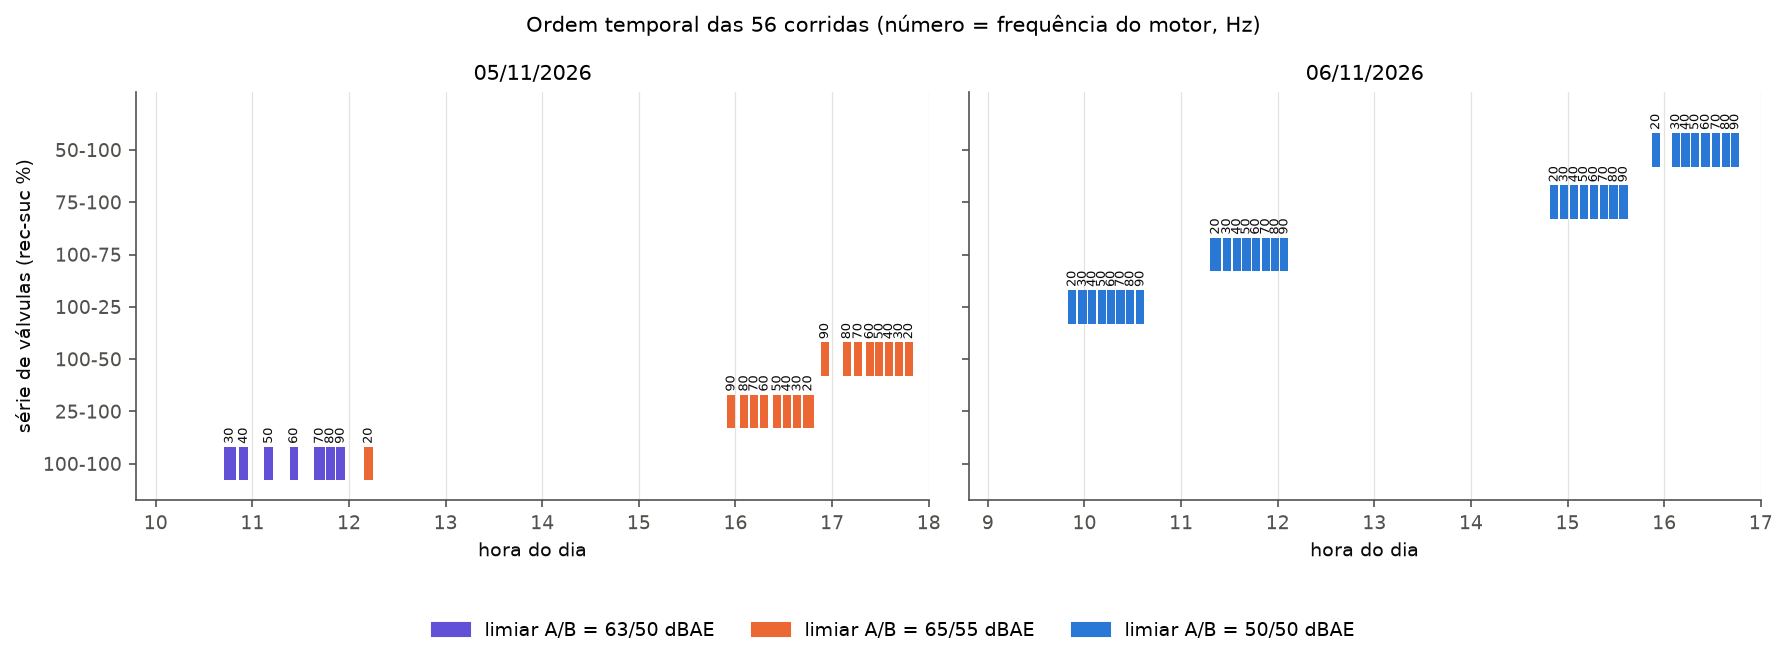
\includegraphics[width=\textwidth]{fig_ordem_temporal.png}
	\caption{Ordem temporal das 56 corridas. Cada barra é uma corrida de cerca de 5\,min; o número acima dela é a frequência do motor e a cor indica o limiar de detecção usado na sessão.}
	\label{fig:ordem}
\end{figure}

\begin{table}[htbp]
	\centering
	\caption{Séries de válvulas, horários, sentido da varredura de frequência e limiares.}
	\label{tab:ordem}
	\small
	\begin{tabular}{llll}
		\toprule
		\textbf{Série} & \textbf{Dia e horário} & \textbf{Ordem das freq.} & \textbf{Limiar A/B (dB\(_{\mathrm{AE}}\))} \\
		\midrule
		100-100 & 05/11, 10h42--12h09 & 30\(\rightarrow\)90, depois 20 & 63/50 (20\,Hz: 65/55) \\
		25-100 & 05/11, 15h54--16h41 & 90\(\rightarrow\)20 & 65/55 \\
		100-50 & 05/11, 16h52--17h45 & 90\(\rightarrow\)20 & 65/55 \\
		100-25 & 06/11, 09h49--10h32 & 20\(\rightarrow\)90 & 50/50 \\
		100-75 & 06/11, 11h17--12h01 & 20\(\rightarrow\)90 & 50/50 \\
		75-100 & 06/11, 14h49--15h32 & 20\(\rightarrow\)90 & 50/50 \\
		50-100 & 06/11, 15h52--16h41 & 20\(\rightarrow\)90 & 50/50 \\
		\bottomrule
	\end{tabular}
\end{table}

% =======================================================================================================
\section{Qualidade dos dados}
\label{sec:qualidade}

Antes de modelar, os registros foram inspecionados. Cinco características condicionam toda a análise.

\paragraph{Saturação.} Com 34\,dB de ganho, 69,8\,\% dos \textit{hits} têm o indicador SAT ativo. A partir de 40 a 50\,Hz, praticamente todos os \textit{hits} dos dois canais saturam, e a amplitude acumula-se no fundo de escala, 102,8\,dB\(_{\mathrm{AE}}\) (Figuras~\ref{fig:exemplo}, \ref{fig:amplitude} e~\ref{fig:mapas}). Nessa faixa, a amplitude de pico deixa de discriminar as condições.

\paragraph{Duração máxima.} 17,8\,\% dos \textit{hits}, quase todos no canal A, atingiram a duração máxima de 100\,ms e foram encerrados pelo MAXDUR. São trechos de emissão contínua, coerentes com ruído de escoamento ou cavitação. A fração MAXDUR do canal A varia entre condições sem ordem simples com a frequência (Figura~\ref{fig:mapas}).

\paragraph{Rearme e cadência dos \textit{hits}.} O indicador ROVL está ativo em 100\,\% dos \textit{hits}, nos dois canais e em todas as corridas. No extrator, ROVL marca um cruzamento do limiar durante o bloqueio re-armável (HLT), que reinicia a espera. Com emissão quase contínua, isso ocorre em todo \textit{hit}, e o indicador não separa nada nestes dados. Além disso, os \textit{hits} de cada canal chegam espaçados em cerca de 0,1\,s, ou cerca de 0,2\,s depois de um \textit{hit} com MAXDUR (Figura~\ref{fig:intervalo}). O canal B registra de 9,5 a 9,9 \textit{hits}/s em quase todas as condições. Essa cadência é compatível com um bloqueio que se estende enquanto houver cruzamentos, até cerca de 100\,ms. O detector passa, então, a amostrar o sinal contínuo a cerca de 10\,Hz. A consequência é que a taxa de \textit{hits} não mede a atividade acústica: ela é função da duração do \textit{hit}. O limite de cerca de 100\,ms não foi confirmado no HDL da versão ensaiada.

\paragraph{Limiar variável.} O limiar mudou entre sessões: 63/50, 65/55 e 50/50\,dB\(_{\mathrm{AE}}\) nos canais A/B (Tabela~\ref{tab:ordem}). Aplicar um corte comum no maior limiar (65,1/55,0\,dB\(_{\mathrm{AE}}\)) removeria apenas 0,001\,\% dos \textit{hits}, porque os picos ficam quase sempre muito acima de qualquer dos limiares. O efeito do limiar está na duração, nas contagens e na energia, que o FPGA mede acima do limiar da sessão, e não pode ser corrigido depois.

\paragraph{Tempo.} A coluna \texttt{timestamp} está zerada. Usou-se o tempo de chegada no computador, \texttt{rx\_time\_s}, cuja resolução é suficiente para janelas de segundos.

\begin{figure}[htbp]
	\centering
	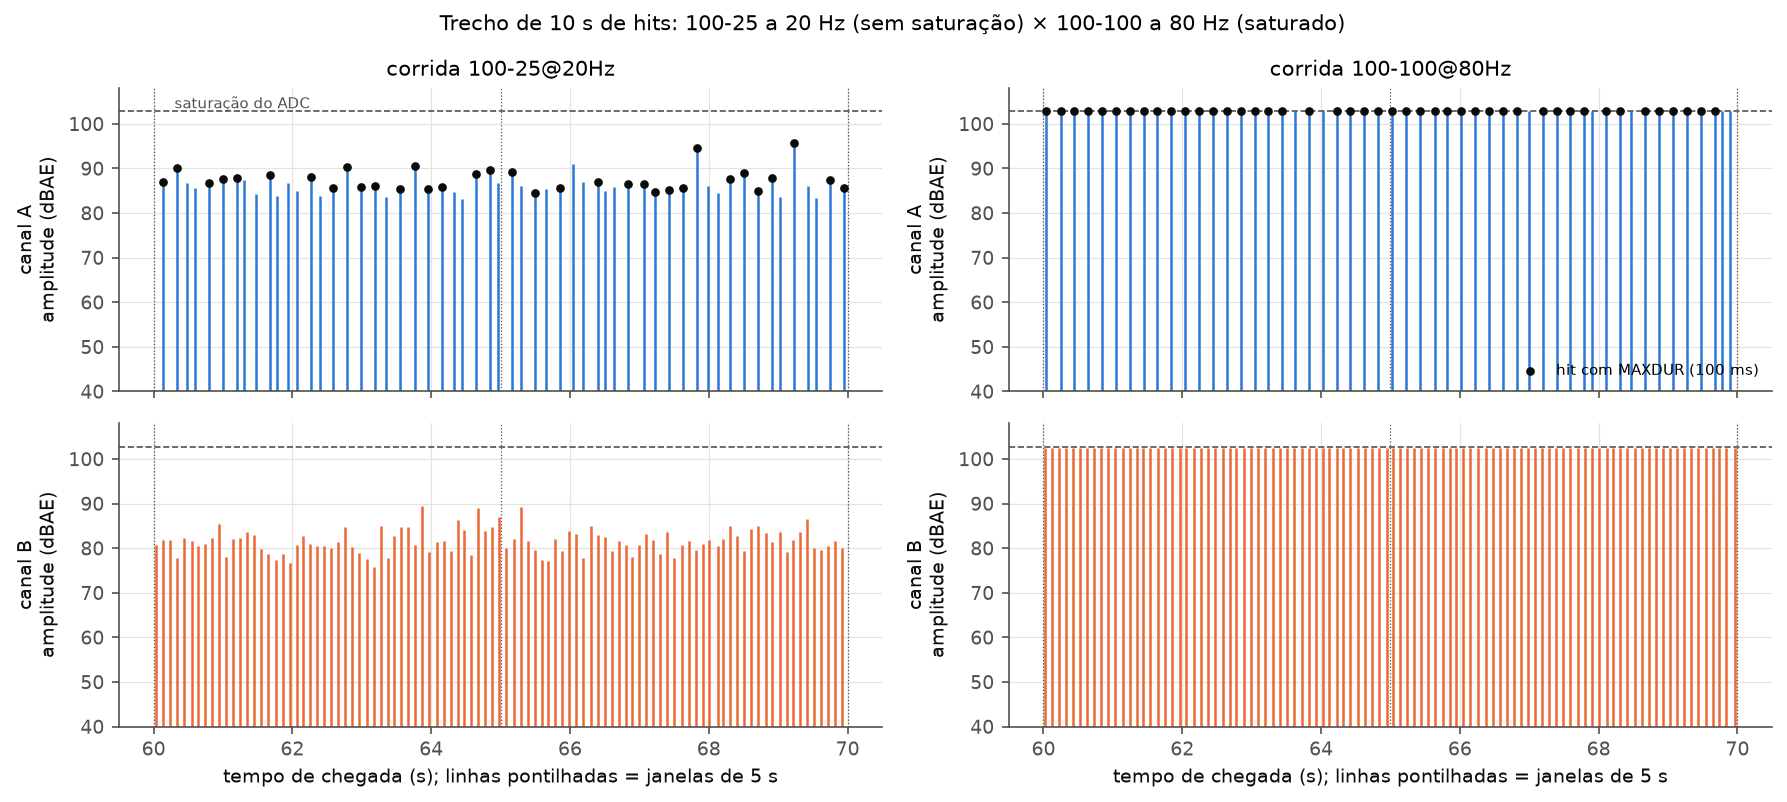
\includegraphics[width=\textwidth]{fig_exemplo_hits.png}
	\caption{Trechos de 10\,s de \textit{hits} em duas corridas. A 20\,Hz (esquerda), as amplitudes variam e não há saturação. A 80\,Hz (direita), todos os \textit{hits} estão no fundo de escala e quase todos os do canal A atingem a duração máxima (pontos pretos). As linhas pontilhadas marcam as janelas de 5\,s.}
	\label{fig:exemplo}
\end{figure}

\begin{figure}[htbp]
	\centering
	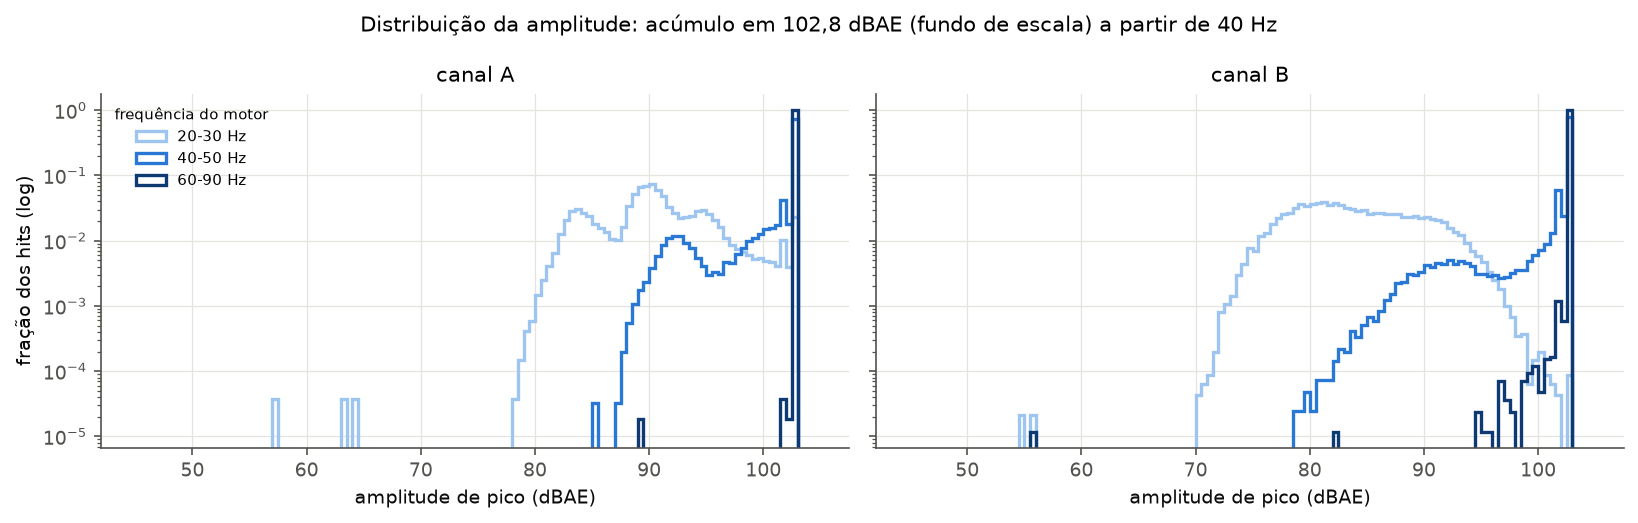
\includegraphics[width=\textwidth]{fig_amplitude_saturacao.png}
	\caption{Distribuição da amplitude de pico por faixa de frequência do motor. A partir de 40\,Hz, a maior parte dos \textit{hits} acumula-se em 102,8\,dB\(_{\mathrm{AE}}\) (saturação do ADC).}
	\label{fig:amplitude}
\end{figure}

\begin{figure}[htbp]
	\centering
	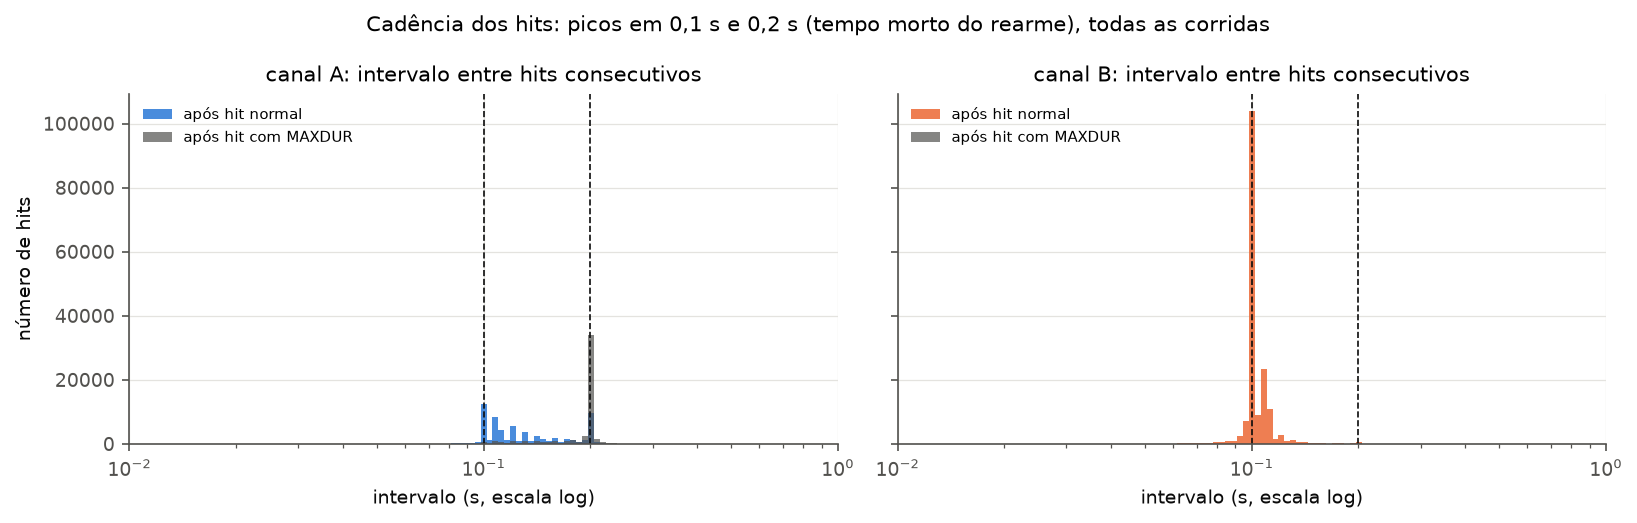
\includegraphics[width=\textwidth]{fig_intervalo_hits.png}
	\caption{Intervalo entre \textit{hits} consecutivos do mesmo canal, em todas as corridas. Os picos em 0,1\,s (após \textit{hit} normal) e 0,2\,s (após \textit{hit} de 100\,ms com MAXDUR) indicam cadência imposta pelo tempo morto do rearme, e não pela atividade acústica.}
	\label{fig:intervalo}
\end{figure}

\begin{figure}[htbp]
	\centering
	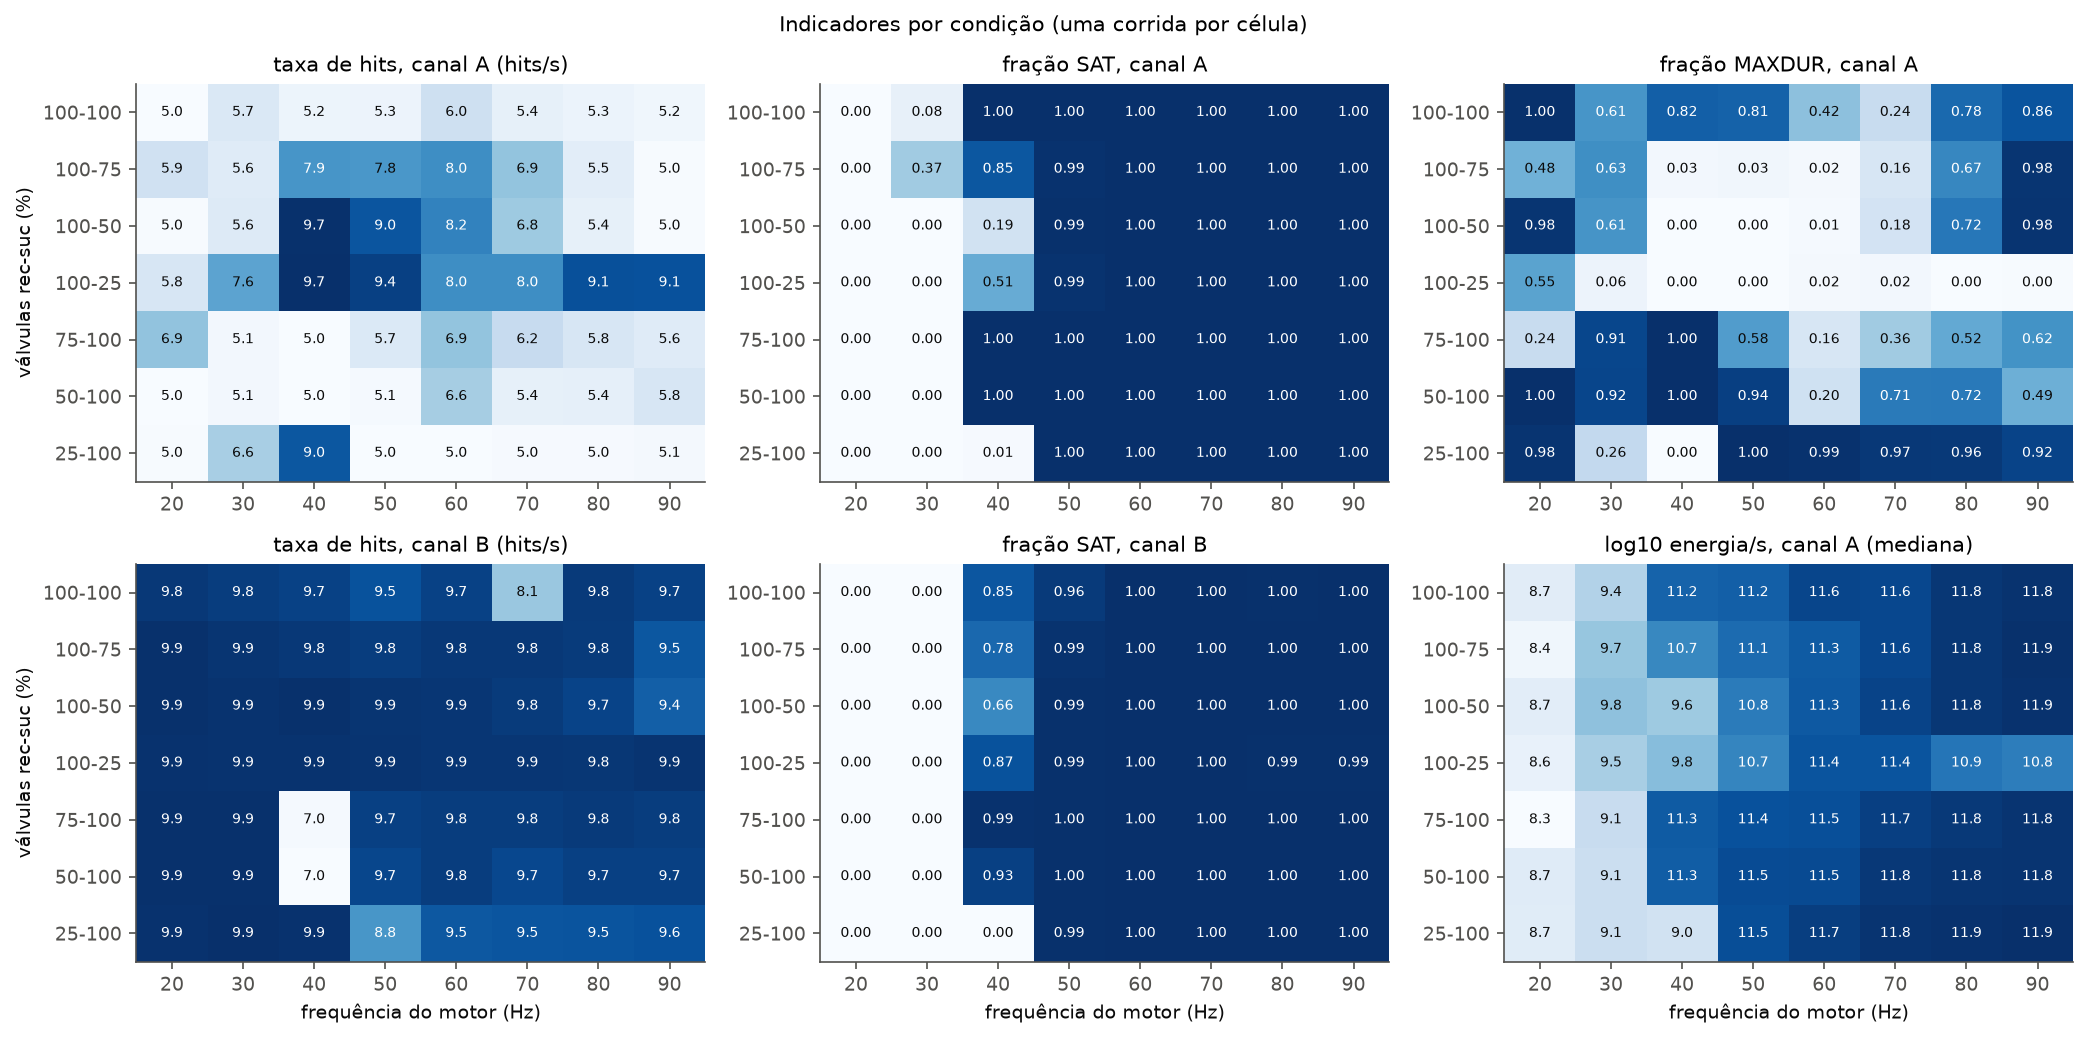
\includegraphics[width=\textwidth]{fig_mapas_condicao.png}
	\caption{Indicadores por condição, um valor por corrida: taxa de \textit{hits}, fração de \textit{hits} saturados (SAT), fração com duração máxima (MAXDUR) e mediana de \(\log_{10}\) da energia por segundo no canal A.}
	\label{fig:mapas}
\end{figure}

% =======================================================================================================
\section{Descritores por janela}
\label{sec:descritores}

A cavitação e o ruído de escoamento são fenômenos quase contínuos. Classificar \textit{hits} isolados faria pouco sentido, porque um \textit{hit} individual não carrega a condição e \textit{hits} vizinhos são redundantes. Os \textit{hits} foram, então, agregados em janelas consecutivas de duração \(T_w = 5\)\,s, sem sobreposição. O resultado são 3\,540 janelas, cerca de 63 por corrida, com aproximadamente 25 a 50 \textit{hits} por canal em cada uma.

Para cada janela e cada canal, calcularam-se 18 descritores, 36 no total.

\textbf{Com todos os \textit{hits} do canal}, cinco descritores:
\begin{itemize}
	\item a taxa de \textit{hits};
	\item a fração saturada (SAT);
	\item a fração com duração máxima (MAXDUR);
	\item o logaritmo da energia total por segundo,
	\begin{equation}
		E_s = \log_{10}\!\Big(\frac{1}{T_w}\sum_{i\in w} E_i + 1\Big),
		\label{eq:energia_s}
	\end{equation}
	que inclui os \textit{hits} contínuos e funciona como um indicador de nível RMS;
	\item a frequência média \(\mathrm{FM} = N_{\mathrm{cont}}/t_{\mathrm{dur}}\), em mediana.
\end{itemize}

\textbf{Só com os \textit{hits} sem MAXDUR}, cuja duração não foi truncada, treze descritores:
\begin{itemize}
	\item média e percentis 10, 50 e 90 da amplitude;
	\item percentis 50 e 90 de \(\log_{10}\) da energia, da duração e das contagens;
	\item mediana de \(\log_{10}\) do tempo de subida;
	\item mediana da frequência média;
	\item mediana de \(\log_{10}\) de RA,
	\begin{equation}
		\mathrm{RA} = \frac{t_{\mathrm{sub}}\ [\mathrm{ms}]}{A_{\mathrm{pico}}\ [\mathrm{V}]},
		\label{eq:ra}
	\end{equation}
	com a amplitude em volts no sensor \cite{ohno2010}.
\end{itemize}

O logaritmo atenua a assimetria de energia, duração e contagens. Janelas sem \textit{hits} normais (6,7\,\% dos valores) ficam com descritores faltantes, imputados pela mediana. Imputação e padronização (média zero, variância unitária) são ajustadas apenas no treino de cada fold.

As Figuras~\ref{fig:box_freq} e~\ref{fig:box_valv} mostram a distribuição de seis descritores por frequência e por válvula. A energia por segundo cresce de forma monotônica com a frequência e estabiliza a partir de cerca de 60\,Hz. A frequência média do canal A cai de 120 a 220\,kHz, em 20\,Hz, para menos de 50\,kHz a partir de 50\,Hz, quando os \textit{hits} longos dominam. Por válvula, as diferenças são menores que a dispersão entre frequências. As exceções são as séries 100-25 e 25-100, que se destacam na fração MAXDUR do canal A: quase nula na primeira e quase total na segunda, acima de 50\,Hz. A Figura~\ref{fig:desc_cond} resume as medianas por corrida.

\begin{figure}[htbp]
	\centering
	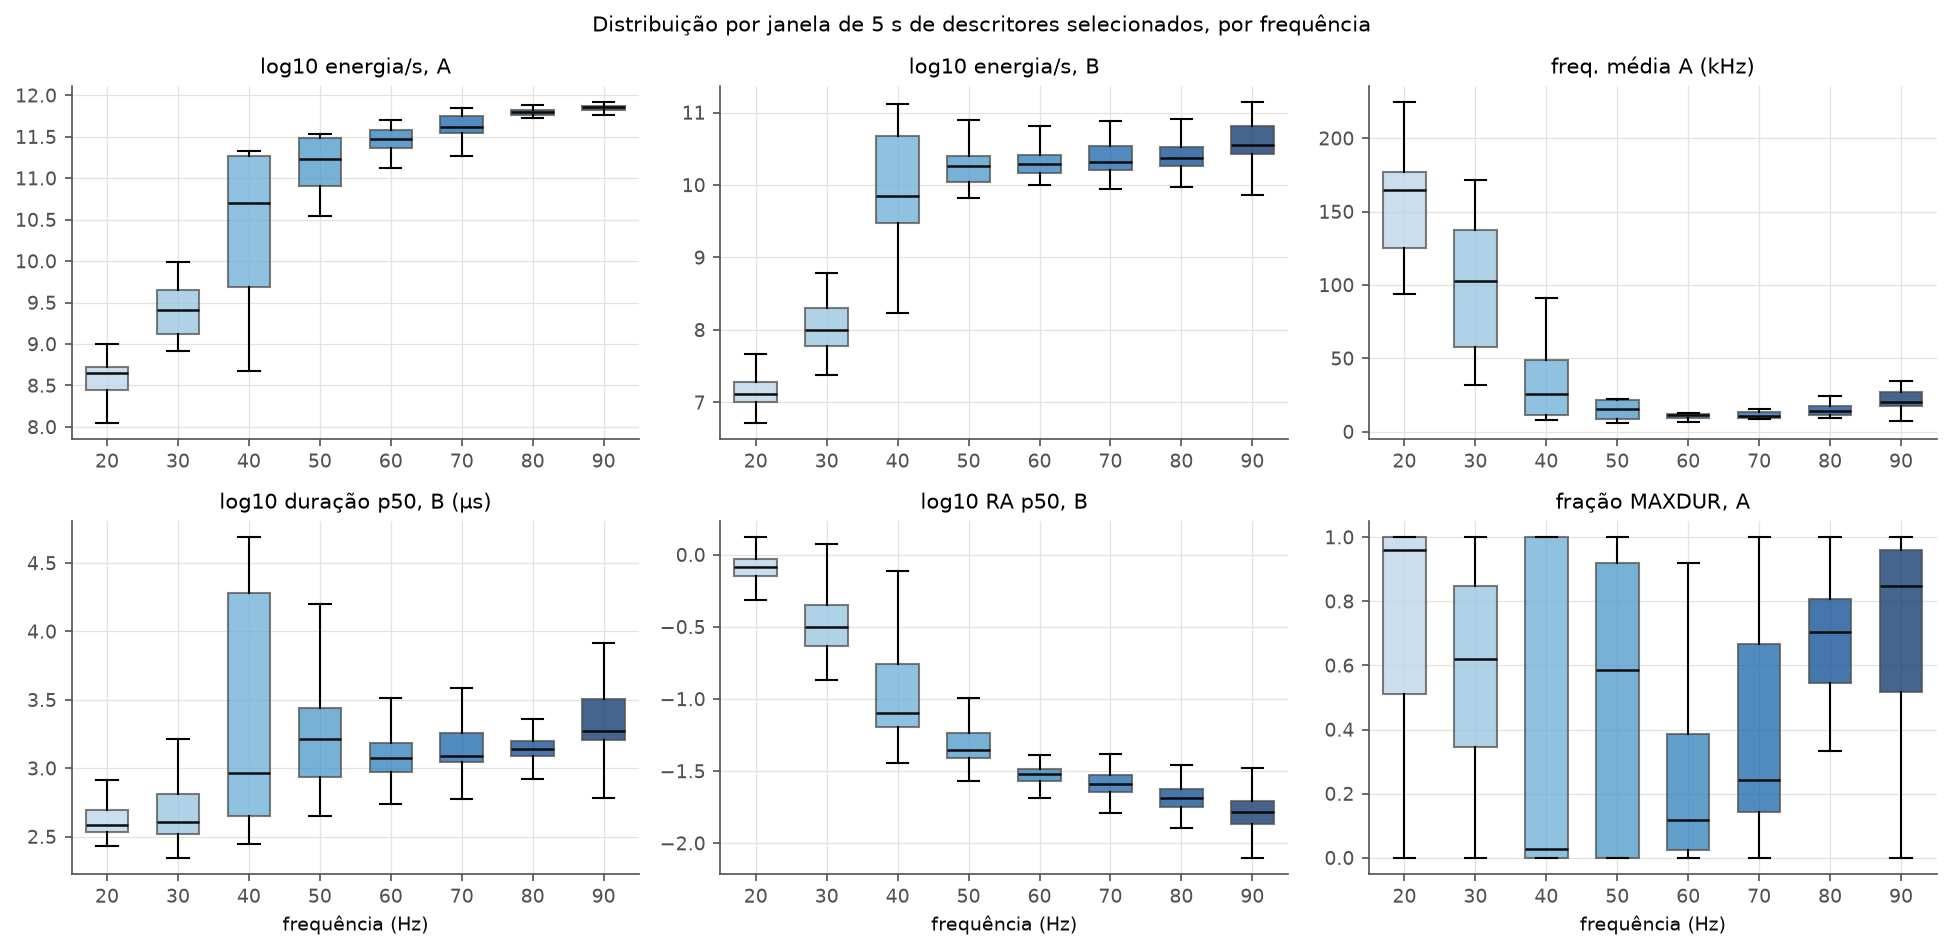
\includegraphics[width=\textwidth]{fig_boxplot_por_frequencia.png}
	\caption{Distribuição, por janela de 5\,s, de seis descritores em função da frequência do motor (todas as configurações de válvula agrupadas).}
	\label{fig:box_freq}
\end{figure}

\begin{figure}[htbp]
	\centering
	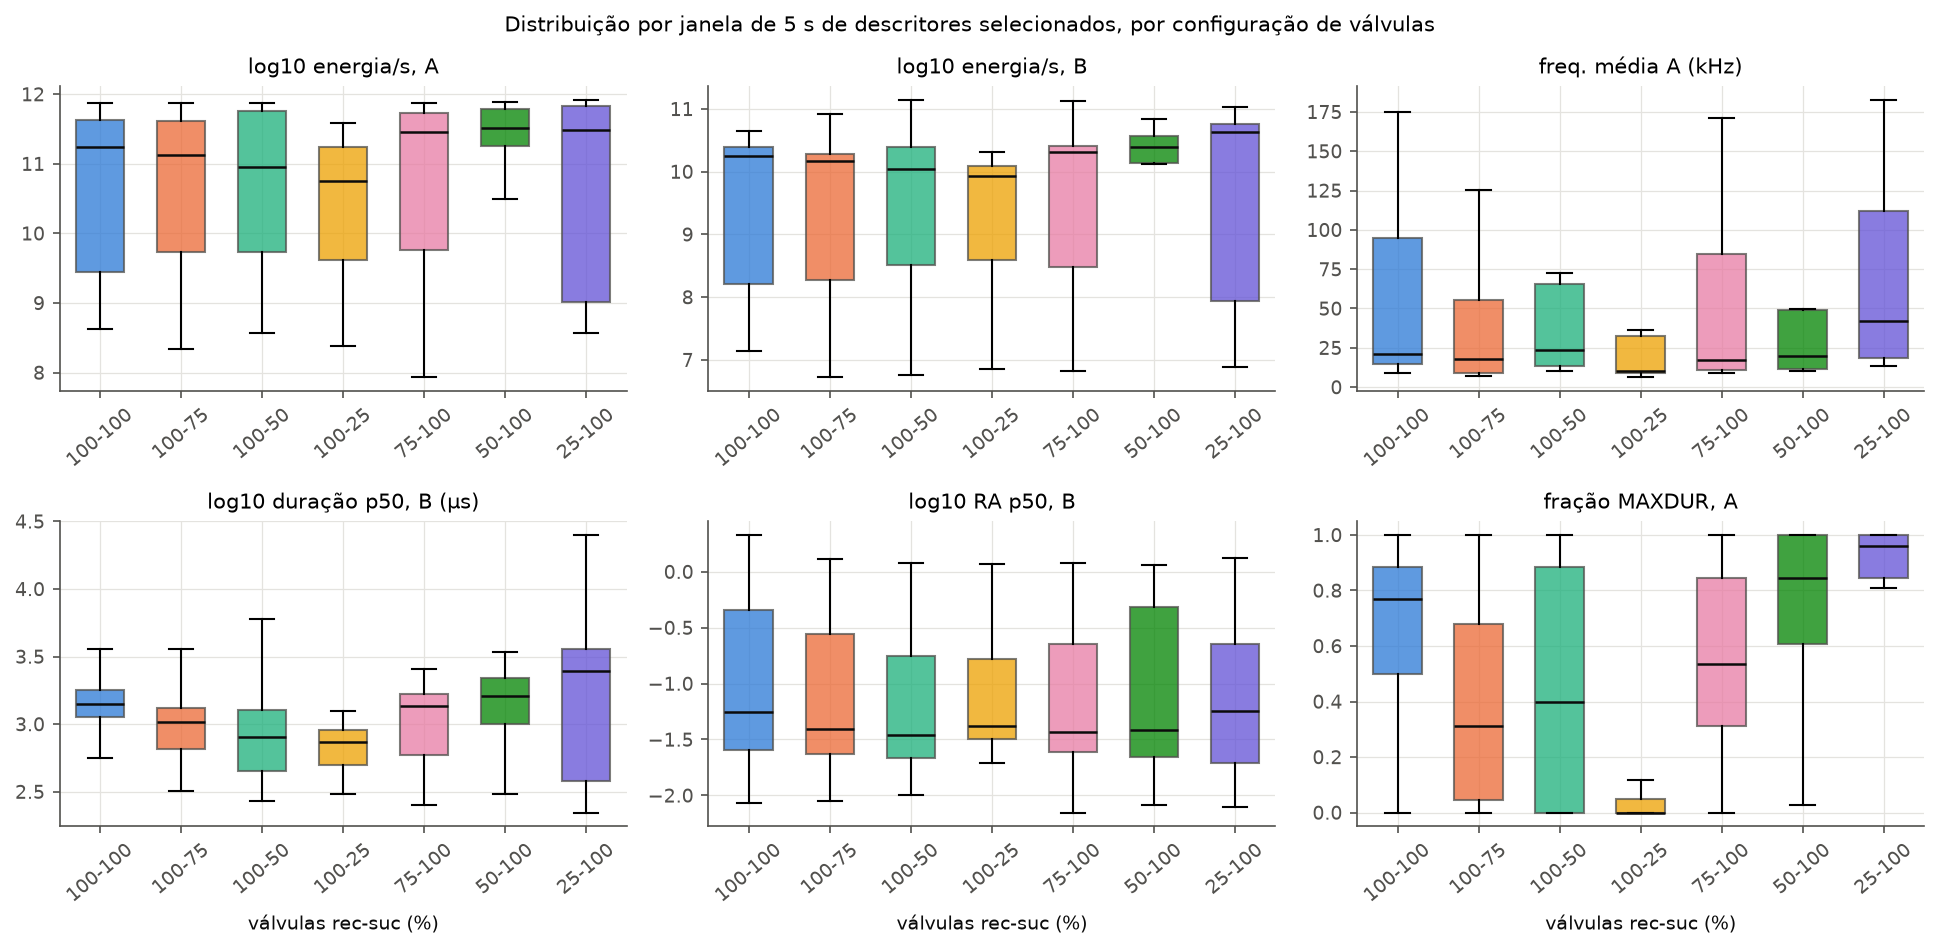
\includegraphics[width=\textwidth]{fig_boxplot_por_valvula.png}
	\caption{Os mesmos descritores da Figura~\ref{fig:box_freq} em função da configuração das válvulas (todas as frequências agrupadas).}
	\label{fig:box_valv}
\end{figure}

\begin{figure}[htbp]
	\centering
	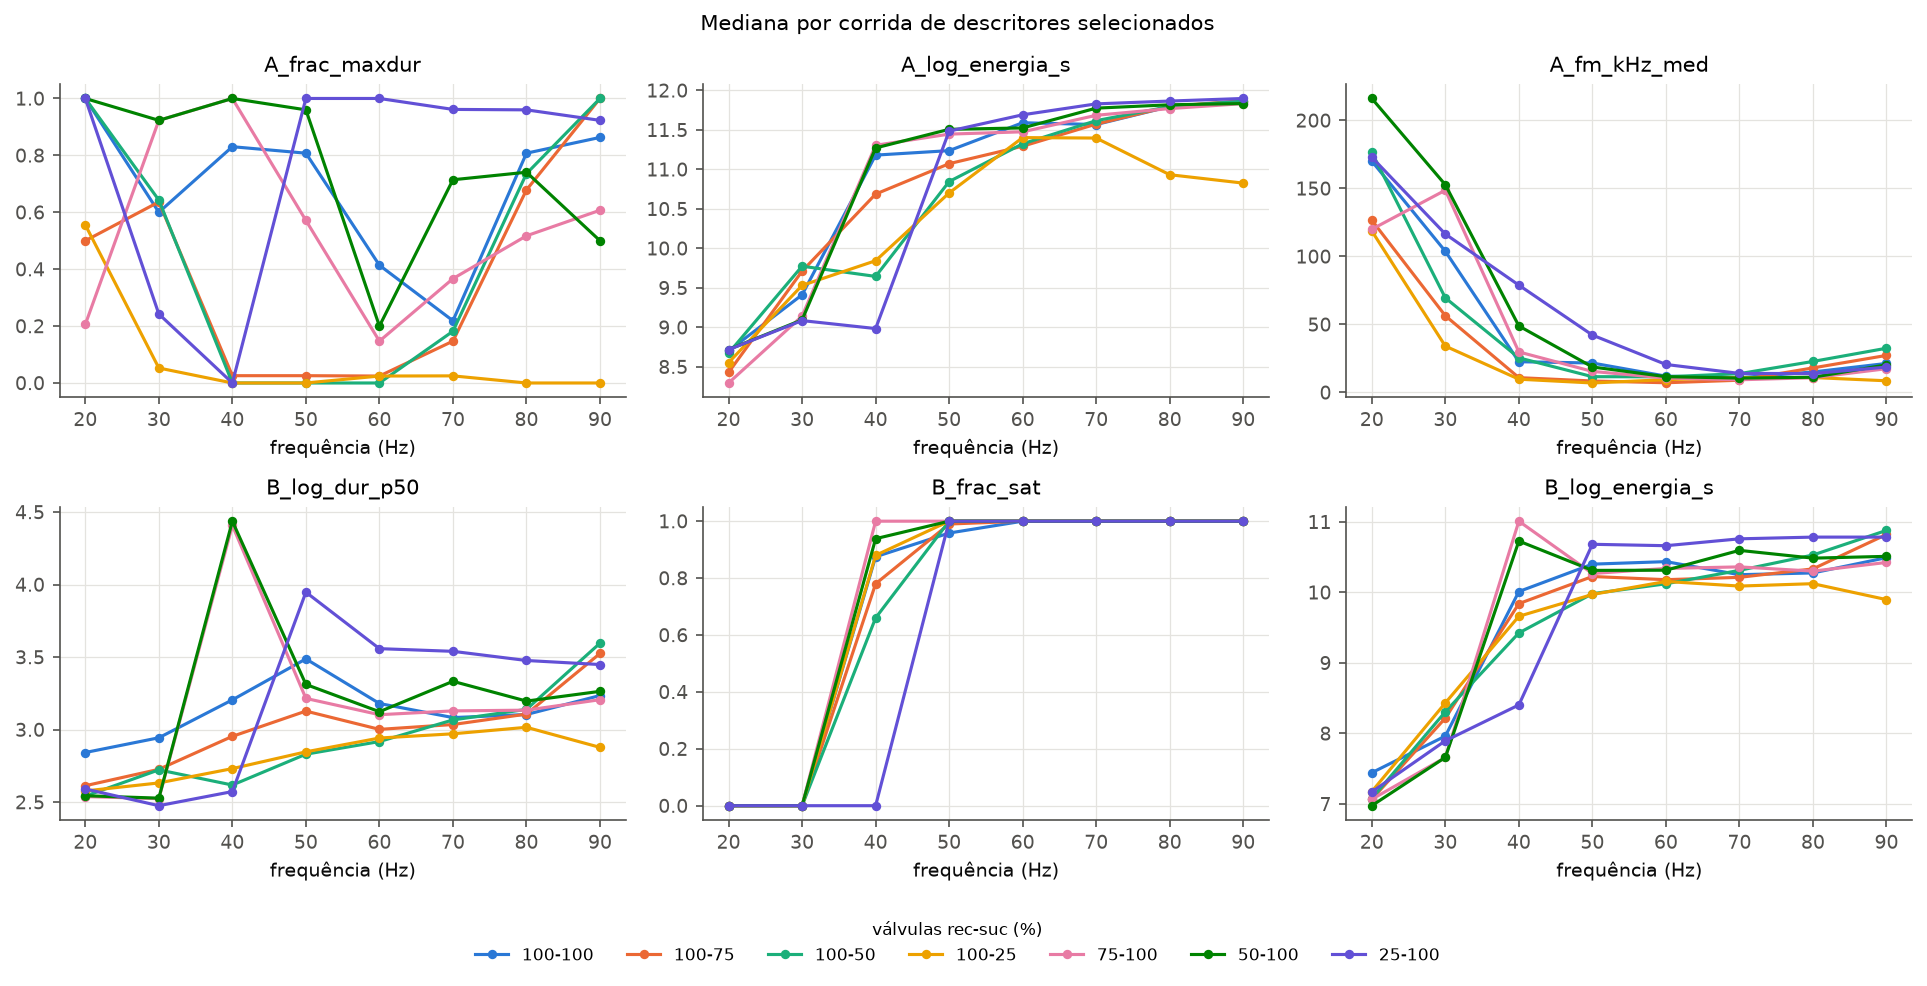
\includegraphics[width=\textwidth]{fig_descritores_por_condicao.png}
	\caption{Mediana por corrida de descritores selecionados em função da frequência, uma curva por configuração de válvulas.}
	\label{fig:desc_cond}
\end{figure}

% =======================================================================================================
\section{Método}
\label{sec:metodo}

\subsection{Alvos}

\paragraph{Frequência.} A frequência do motor é uma grandeza ordenada. Foi tratada como \textbf{regressão}, e a leitura ordinal foi obtida arredondando a previsão ao nível mais próximo entre 20 e 90\,Hz. Assim, errar 40\,Hz por 50\,Hz custa menos que errar por 90\,Hz, o que não ocorreria com oito classes independentes.

\paragraph{Válvulas.} Como o delineamento é cruzado, só existem 7 das 16 combinações possíveis de recalque e sucção. A configuração foi modelada como \textbf{uma classe com 7 níveis}, equilibrada com 8 corridas por classe. Os acertos em \% recalque e \% sucção foram derivados da classe prevista. Dois classificadores independentes poderiam prever combinações nunca ensaiadas e teriam classes desbalanceadas, já que 100\,\% aparece em 4 das 7 configurações. Em nenhum caso o problema foi formulado como 56 classes.

\subsection{Modelos}

Três modelos foram comparados, todos com hiperparâmetros fixos e precedidos de imputação e padronização no mesmo \textit{pipeline} (scikit-learn 1.9.1 \cite{pedregosa2011}).

\begin{itemize}
	\item \textbf{MLP}: duas camadas ocultas de 64 e 32 neurônios, ReLU, otimizador Adam, penalidade L2 \(\alpha = 10^{-3}\) e parada antecipada. A parada usa 15\,\% das janelas de treino como validação interna, com paciência de 30 épocas, e restaura os pesos da melhor época \cite{prechelt1998}. Na regressão, o alvo também é padronizado.
	\item \textbf{RF}: 300 árvores, mínimo de 2 amostras por folha e 50\,\% dos descritores por divisão na regressão (\(\sqrt{p}\) na classificação) \cite{breiman2001}.
	\item \textbf{GB}: \textit{HistGradientBoosting}, com 300 iterações na regressão e 200 na classificação, taxa de aprendizado de 0,05 e sem parada antecipada \cite{friedman2001}.
\end{itemize}

A ausência de busca de hiperparâmetros é deliberada. Com 56 corridas, uma busca aninhada teria pouca resolução \cite{varma2006}, e otimizar sobre o próprio teste inflaria os resultados. Os números são, portanto, linhas de base.

\subsection{Validação}

Nenhuma validação sorteia \textit{hits} ou janelas entre treino e teste (Figura~\ref{fig:div_aleat}). Como não há repetições das condições, não foi possível deixar uma repetição de fora. Usaram-se três esquemas, em ordem crescente de independência \cite{roberts2017}:

\begin{description}
	\item[BLOCOS (pseudo-repetição, 5 folds).] Cada corrida é dividida em 5 trechos consecutivos de cerca de 60\,s. No fold \(k\), o \(k\)-ésimo trecho de todas as corridas é o teste, e o restante é o treino. Uma janela de cada lado do trecho de teste é excluída para reduzir a dependência entre janelas contíguas (Figura~\ref{fig:div_blocos}). A mesma corrida aparece no treino e no teste.
	\item[LORO (\textit{leave-one-run-out}, 56 folds).] Uma corrida inteira é o teste. Sua frequência aparece no treino com outras válvulas, e sua configuração aparece com outras frequências (Figura~\ref{fig:div_loro}). Este é o teste de generalização para uma condição não vista.
	\item[LOSO (\textit{leave-one-series-out}, 7 folds, só frequência).] Uma série de válvulas inteira, isto é, uma sessão contínua, é o teste (Figura~\ref{fig:div_loso}). A classificação das válvulas não é possível aqui, porque a classe testada estaria ausente do treino.
\end{description}

As métricas da frequência são o erro absoluto médio (MAE), o RMSE, o \(R^2\), o acerto do nível exato e o acerto em \(\pm 10\)\,Hz. As das válvulas são a acurácia, a acurácia balanceada, o F1 macro e os acertos de \% recalque e \% sucção. Todas foram calculadas por janela e também por corrida: mediana das previsões para a frequência e voto majoritário para as válvulas.

\begin{figure}[htbp]
	\centering
	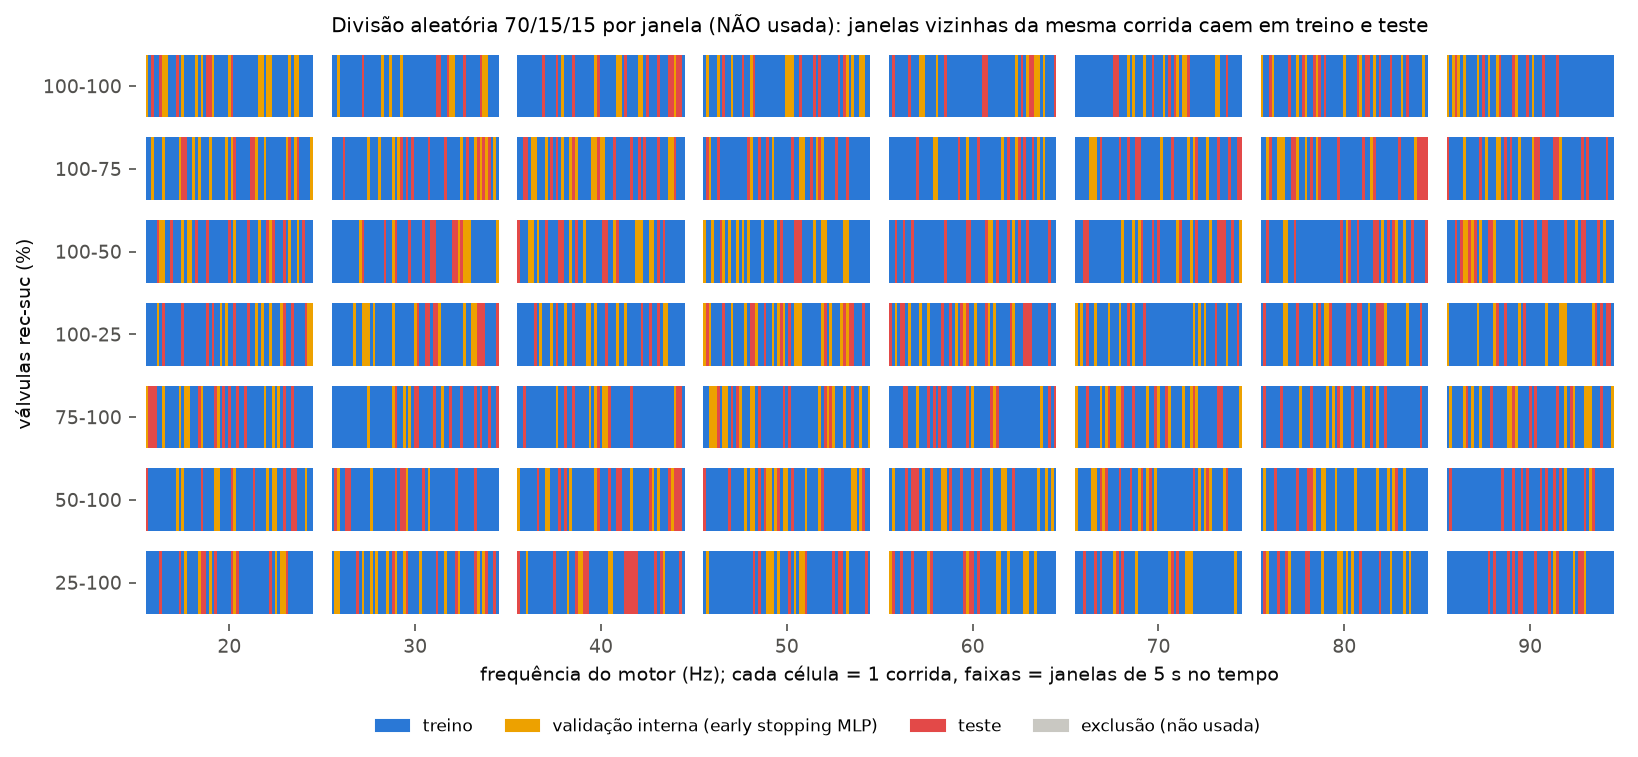
\includegraphics[width=0.92\textwidth]{fig_divisao_aleatoria.png}
	\caption{Divisão aleatória 70/15/15 por janela, \textbf{não} usada. Janelas vizinhas da mesma corrida caem em treino, validação e teste, o que mede a memorização da corrida.}
	\label{fig:div_aleat}
\end{figure}

\begin{figure}[htbp]
	\centering
	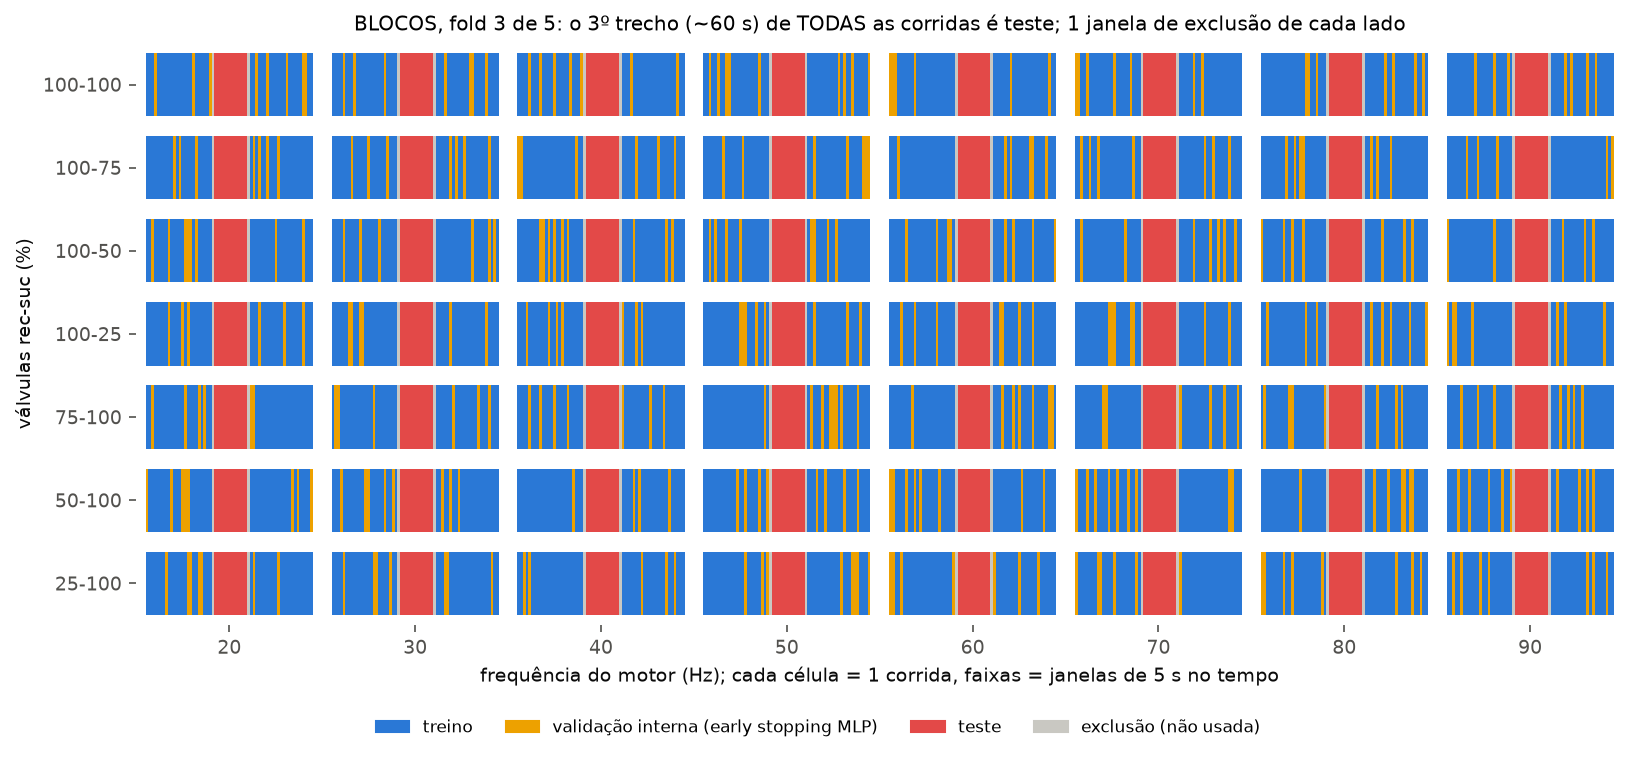
\includegraphics[width=0.92\textwidth]{fig_divisao_blocos.png}
	\caption{Esquema BLOCOS (fold 3 de 5): o terceiro trecho de cada corrida é o teste, com uma janela de exclusão de cada lado. As faixas amarelas são a validação interna da parada antecipada da MLP, sorteada dentro do treino.}
	\label{fig:div_blocos}
\end{figure}

\begin{figure}[htbp]
	\centering
	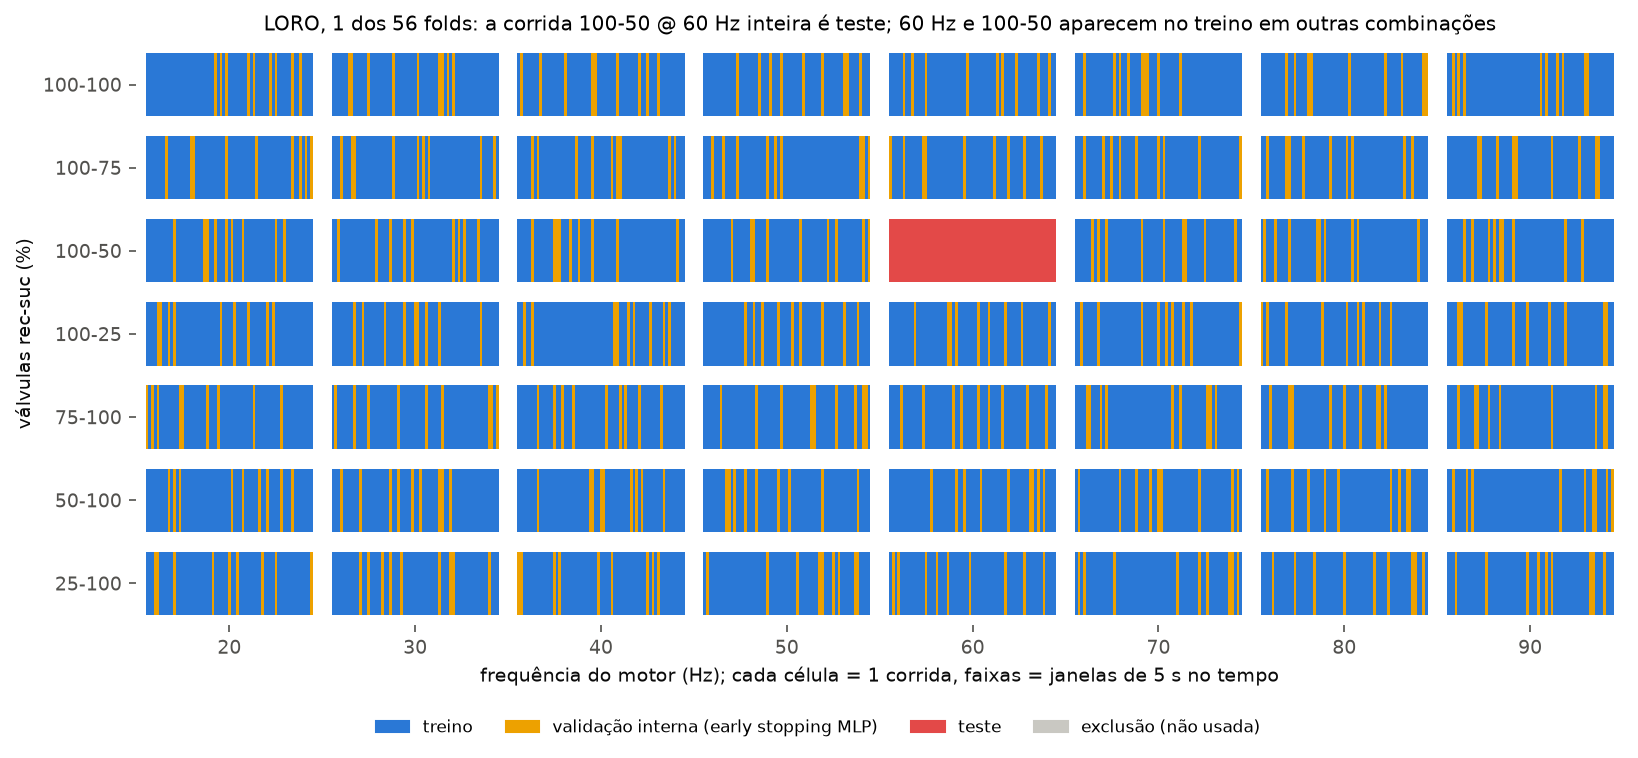
\includegraphics[width=0.92\textwidth]{fig_divisao_loro.png}
	\caption{Esquema LORO (um dos 56 folds): a corrida 100-50 a 60\,Hz inteira é o teste.}
	\label{fig:div_loro}
\end{figure}

\begin{figure}[htbp]
	\centering
	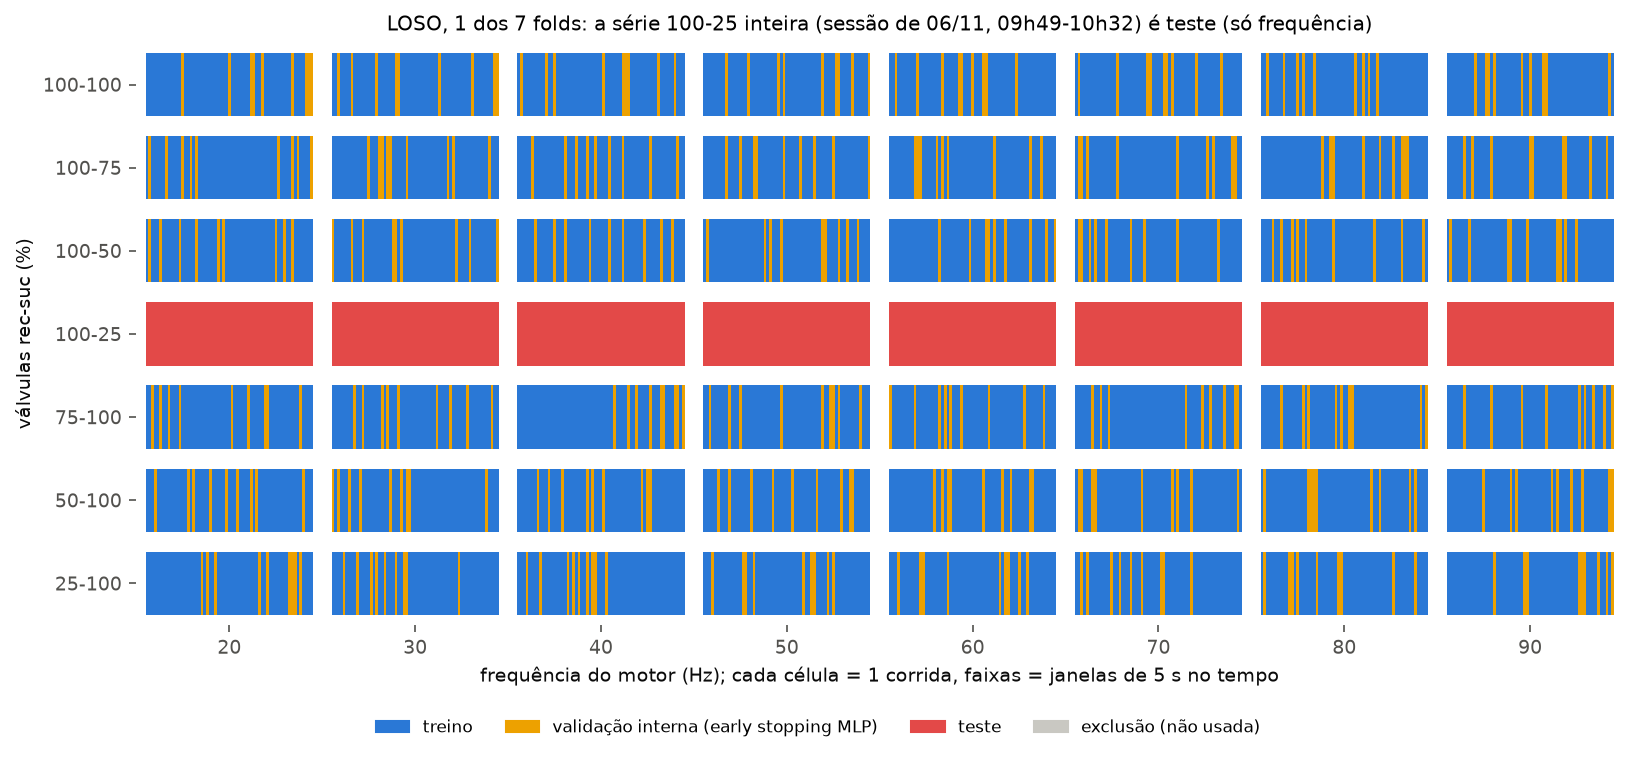
\includegraphics[width=0.92\textwidth]{fig_divisao_loso.png}
	\caption{Esquema LOSO (um dos 7 folds): a série 100-25 inteira é o teste.}
	\label{fig:div_loso}
\end{figure}

% =======================================================================================================
\section{Resultados}
\label{sec:resultados}

\subsection{Frequência do motor}

A Tabela~\ref{tab:freq} e as Figuras~\ref{fig:blocos_loro} a~\ref{fig:conf_loso} resumem os resultados. Com a corrida presente no treino (BLOCOS), o MAE fica entre 1,1 e 2,1\,Hz. Com a corrida ou a série inteira fora do treino, o MAE sobe para 4,2 a 5,6\,Hz, mas 92 a 95\,\% das janelas continuam a até um nível do valor real. Os níveis de 20 e 30\,Hz, sem saturação, são reconhecidos quase sempre. Os erros concentram-se entre níveis vizinhos de 40 a 90\,Hz, onde a saturação achata a amplitude. Por frequência, o MAE em LORO vai de 0,1 a 1,6\,Hz em 20 e 30\,Hz e de 9,5 a 11,5\,Hz em 50\,Hz.

\begin{table}[htbp]
	\centering
	\caption{Frequência do motor: métricas por janela e por corrida. MAE e RMSE em Hz; Nível = acerto da previsão arredondada a 20, 30, \ldots, 90\,Hz; Corrida = acerto do nível usando a mediana das janelas da corrida.}
	\label{tab:freq}
	\small
	\begin{tabular}{llrrrrrr}
		\toprule
		\textbf{Validação} & \textbf{Modelo} & \textbf{MAE} & \textbf{RMSE} & \(\boldsymbol{R^2}\) & \textbf{Nível} & \(\boldsymbol{\pm}\)\textbf{10\,Hz} & \textbf{Corrida} \\
		\midrule
		BLOCOS & MLP & 2,06 & 4,47 & 0,962 & 0,927 & 0,991 & 0,982 \\
		BLOCOS & RF & 1,08 & 2,84 & 0,985 & 0,943 & 0,990 & 0,982 \\
		BLOCOS & GB & 1,16 & 2,98 & 0,983 & 0,952 & 0,988 & 0,982 \\
		\midrule
		LORO & MLP & 5,61 & 10,56 & 0,790 & 0,691 & 0,918 & 0,714 \\
		LORO & RF & 4,85 & 7,87 & 0,883 & 0,612 & 0,942 & 0,589 \\
		LORO & GB & 4,97 & 8,03 & 0,879 & 0,608 & 0,949 & 0,625 \\
		\midrule
		LOSO & MLP & 5,09 & 8,93 & 0,850 & 0,698 & 0,939 & 0,768 \\
		LOSO & RF & 4,23 & 7,80 & 0,885 & 0,691 & 0,951 & 0,679 \\
		LOSO & GB & 4,21 & 7,72 & 0,888 & 0,701 & 0,951 & 0,714 \\
		\bottomrule
	\end{tabular}
\end{table}

RF e GB têm MAE menor, enquanto a MLP acerta mais o nível exato em LORO (69\,\% contra 61\,\%). Com 56 corridas, nenhuma das diferenças entre modelos é conclusiva.

Em LOSO (Figura~\ref{fig:mae_fold}), o pior caso é a série 100-25, com sucção a 25\,\% e MAE de 9,9 a 10,6\,Hz. Essa série é a mais distinta: a energia do canal A cai acima de 70\,Hz e a fração MAXDUR é praticamente nula, o que é coerente com outro regime de escoamento na sucção estrangulada. As séries ensaiadas em ordem decrescente (25-100 e 100-50) têm MAE de 3,6 a 7,9\,Hz. A previsão da frequência, portanto, não se apoia apenas no sentido crescente da varredura.

Um teste adicional fora do tempo, treinando com as séries de um dia e testando nas do outro (Figura~\ref{fig:oot}), deu MAE de 4,4 a 6,6\,Hz (05/11\(\rightarrow\)06/11) e de 4,0 a 5,7\,Hz (06/11\(\rightarrow\)05/11). Esses valores estão na mesma faixa do LOSO, apesar da troca de dia e de limiar.

\begin{figure}[htbp]
	\centering
	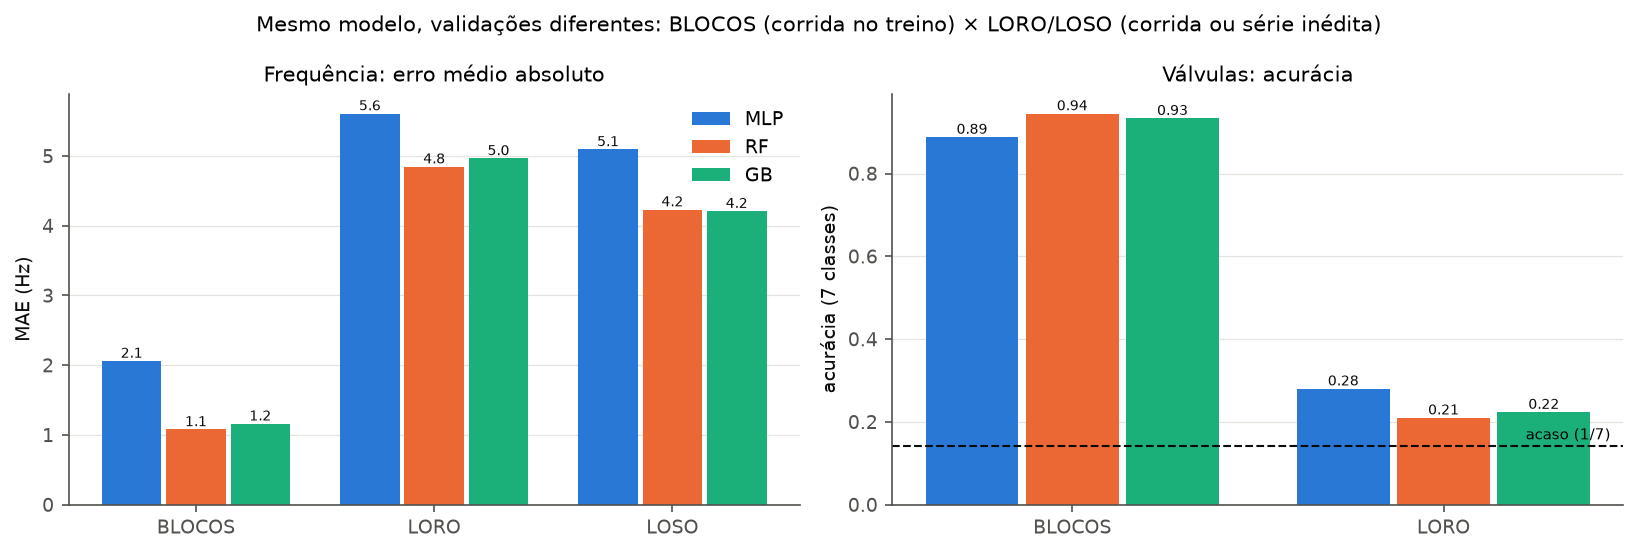
\includegraphics[width=\textwidth]{fig_blocos_vs_loro.png}
	\caption{O mesmo modelo avaliado por validações diferentes. A frequência perde precisão, mas generaliza. As válvulas caem para perto do acaso quando a corrida sai do treino.}
	\label{fig:blocos_loro}
\end{figure}

\begin{figure}[htbp]
	\centering
	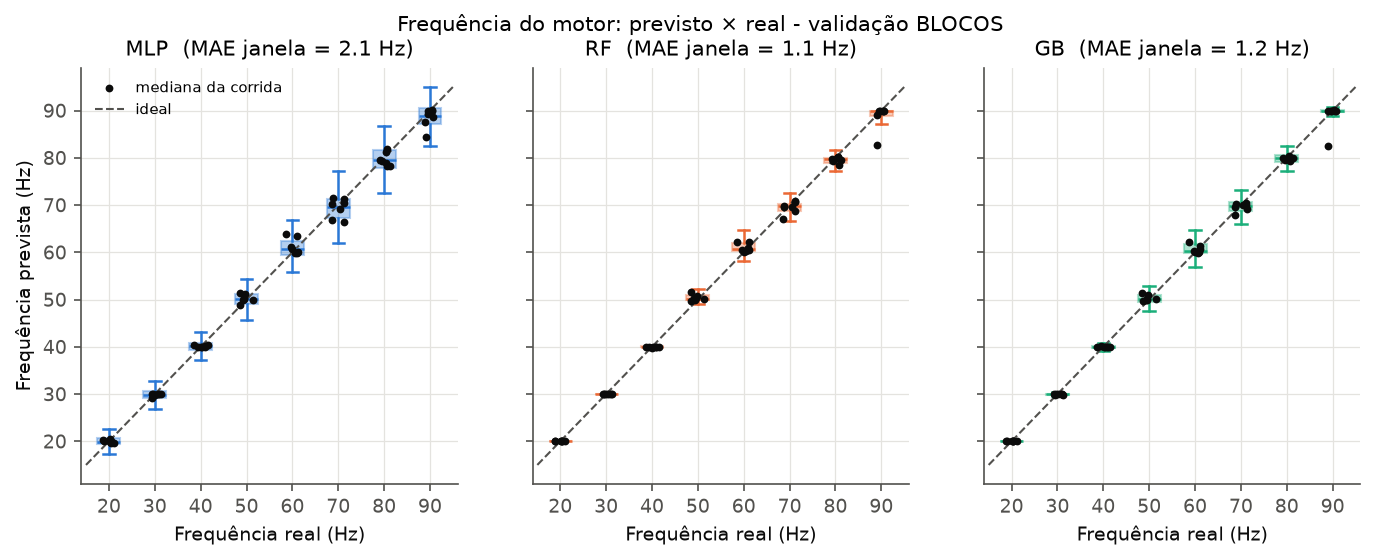
\includegraphics[width=\textwidth]{fig_freq_previsto_real_BLOCOS.png}
	\caption{Frequência prevista \(\times\) real na validação BLOCOS. Caixas: distribuição das janelas; pontos: mediana de cada corrida.}
	\label{fig:pr_blocos}
\end{figure}

\begin{figure}[htbp]
	\centering
	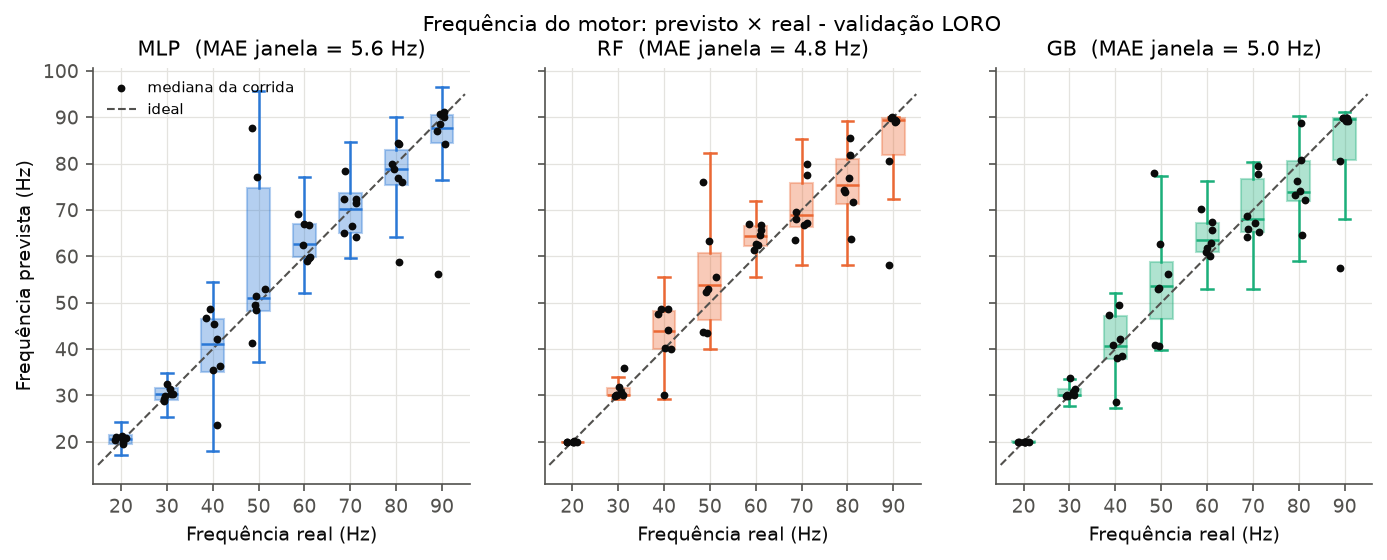
\includegraphics[width=\textwidth]{fig_freq_previsto_real_LORO.png}
	\caption{Frequência prevista \(\times\) real com a corrida deixada de fora (LORO).}
	\label{fig:pr_loro}
\end{figure}

\begin{figure}[htbp]
	\centering
	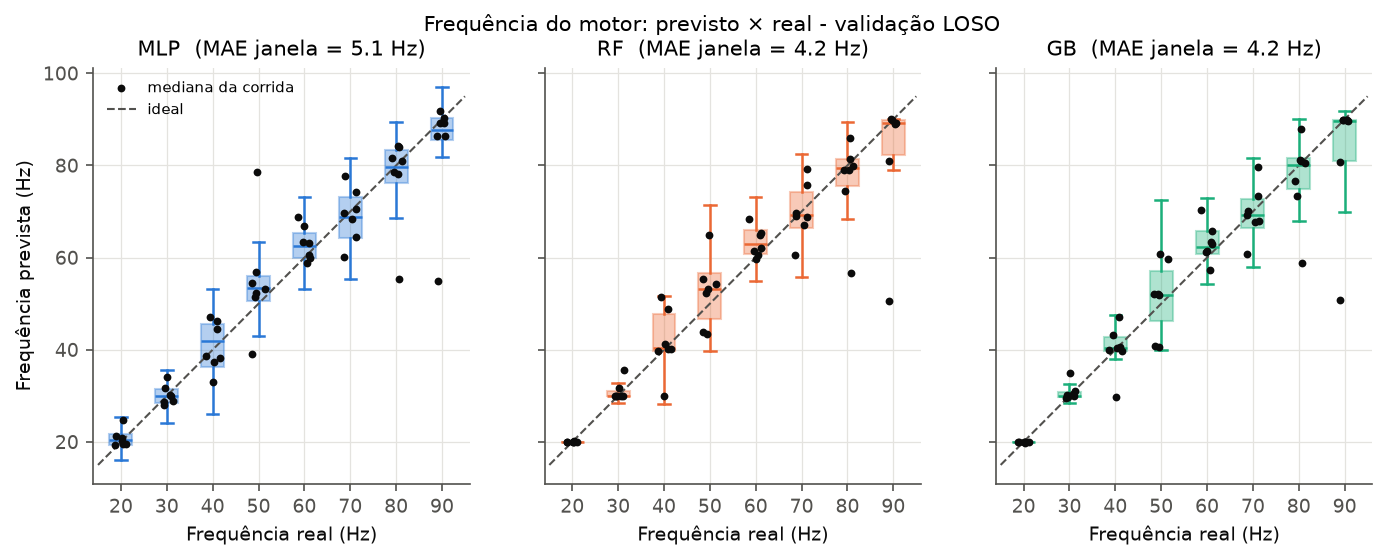
\includegraphics[width=\textwidth]{fig_freq_previsto_real_LOSO.png}
	\caption{Frequência prevista \(\times\) real com a série de válvulas deixada de fora (LOSO).}
	\label{fig:pr_loso}
\end{figure}

\begin{figure}[htbp]
	\centering
	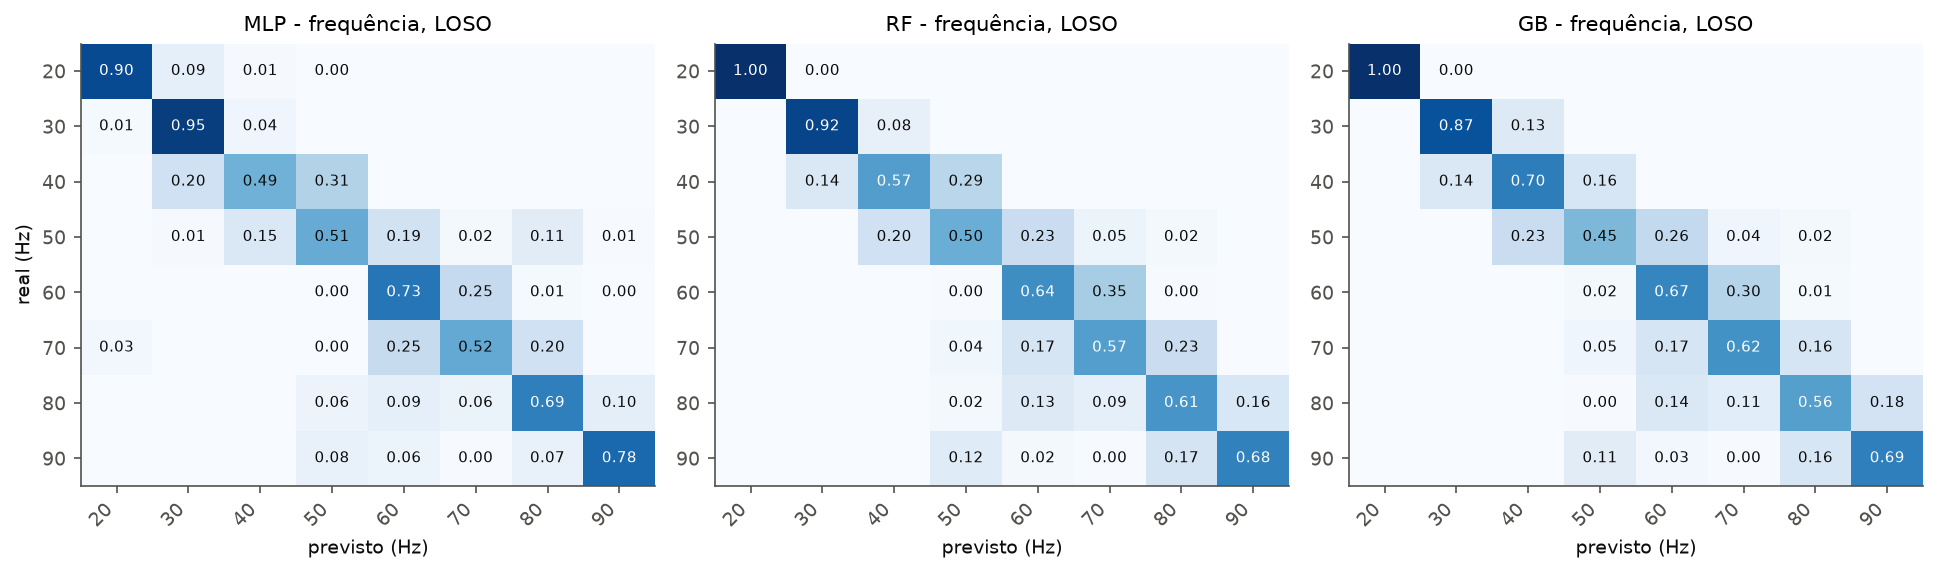
\includegraphics[width=\textwidth]{fig_confusao_LOSO.png}
	\caption{Matrizes de confusão da frequência arredondada em LOSO, com linhas normalizadas.}
	\label{fig:conf_loso}
\end{figure}

\begin{figure}[htbp]
	\centering
	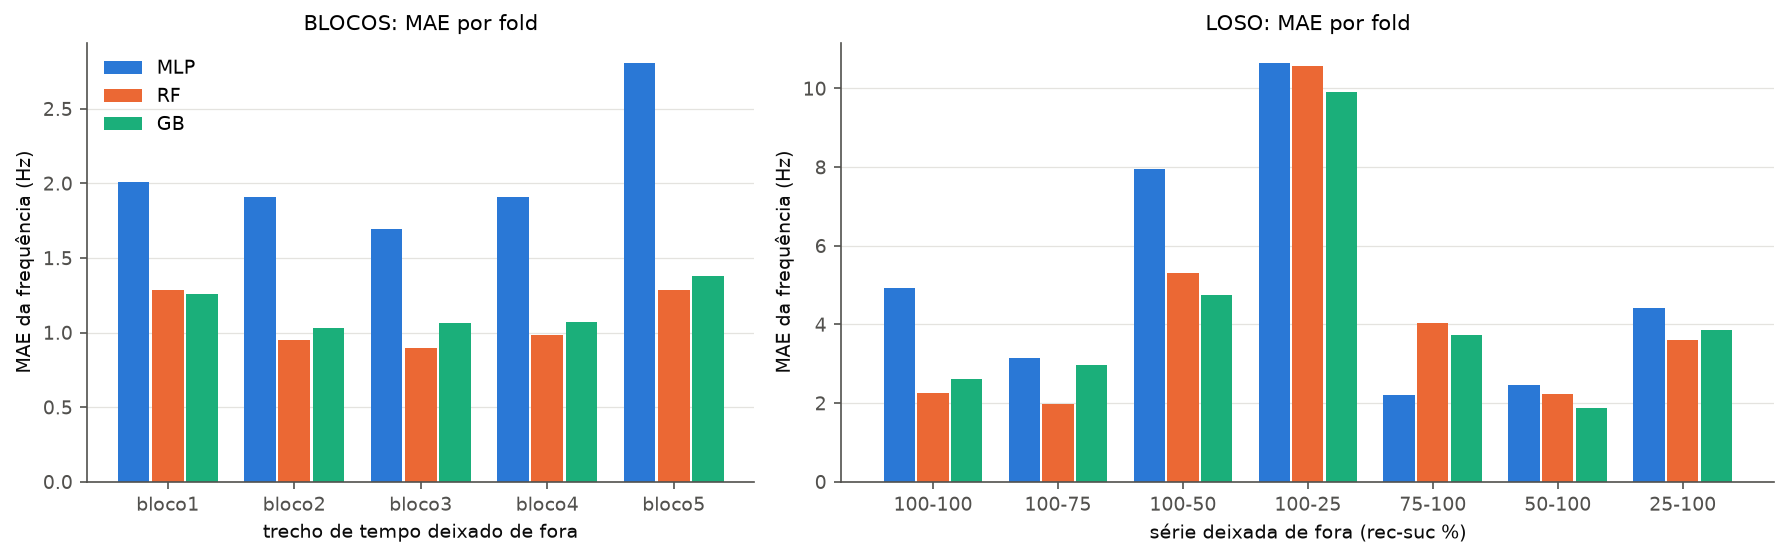
\includegraphics[width=\textwidth]{fig_mae_por_fold.png}
	\caption{MAE da frequência por fold: trechos de tempo em BLOCOS (esquerda) e séries de válvulas em LOSO (direita).}
	\label{fig:mae_fold}
\end{figure}

\begin{figure}[htbp]
	\centering
	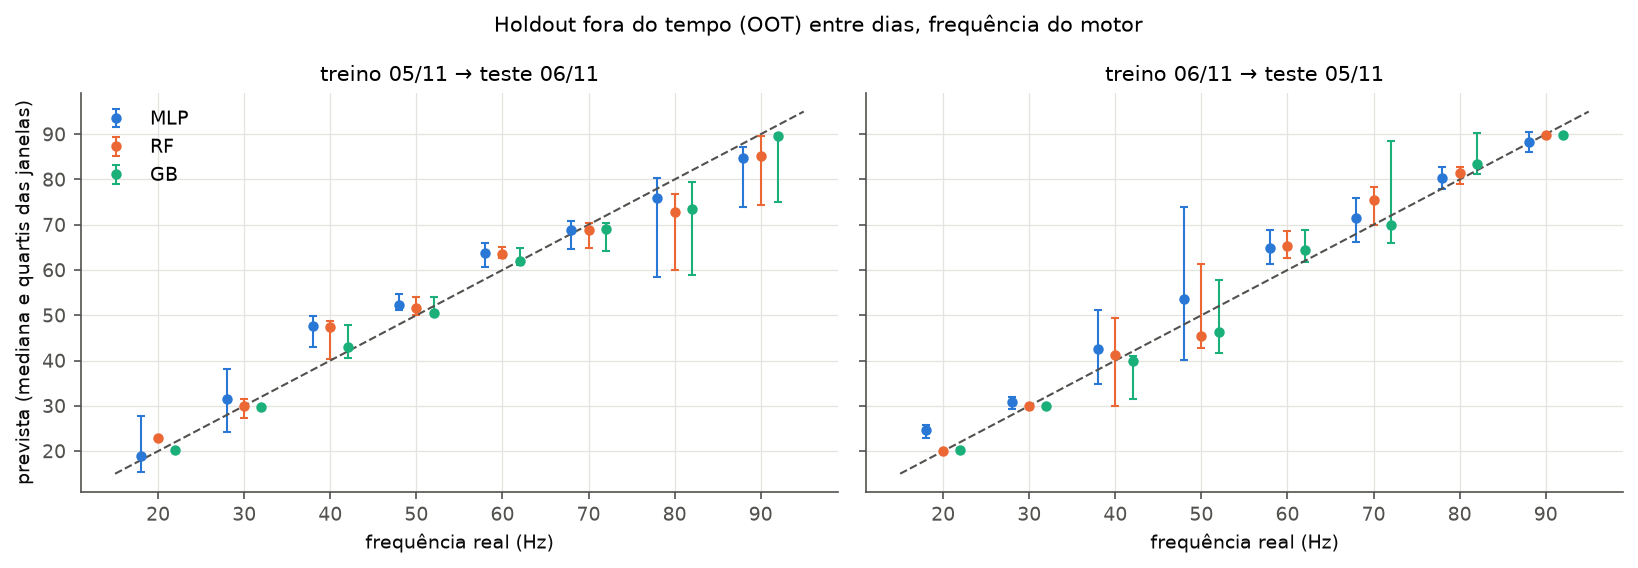
\includegraphics[width=\textwidth]{fig_oot_por_dia.png}
	\caption{Teste fora do tempo entre dias: treino com as séries de um dia e teste nas do outro (mediana e quartis das janelas).}
	\label{fig:oot}
\end{figure}

\subsection{Configuração das válvulas}

A Tabela~\ref{tab:valv} mostra o contraste central do trabalho. Em BLOCOS, as válvulas parecem bem reconhecidas: 89 a 95\,\% por janela e 100\,\% por corrida. Em LORO, a acurácia cai para 21 a 28\,\%, pouco acima do acaso de 14\,\%. Os acertos de \% recalque e \% sucção (53 a 59\,\%) ficam no nível de um classificador que sempre responde 100\,\% (57\,\%).

\begin{table}[htbp]
	\centering
	\caption{Configuração das válvulas (7 classes): acurácia por janela, acurácia balanceada, F1 macro, acerto de \% recalque e \% sucção derivados e acurácia por corrida (voto majoritário).}
	\label{tab:valv}
	\small
	\begin{tabular}{llrrrrrr}
		\toprule
		\textbf{Validação} & \textbf{Modelo} & \textbf{Acurácia} & \textbf{Ac. bal.} & \textbf{F1} & \textbf{\% rec} & \textbf{\% suc} & \textbf{Corrida} \\
		\midrule
		BLOCOS & MLP & 0,888 & 0,888 & 0,888 & 0,919 & 0,946 & 1,000 \\
		BLOCOS & RF & 0,945 & 0,944 & 0,944 & 0,958 & 0,970 & 1,000 \\
		BLOCOS & GB & 0,934 & 0,933 & 0,933 & 0,948 & 0,964 & 1,000 \\
		\midrule
		LORO & MLP & 0,280 & 0,279 & 0,276 & 0,573 & 0,594 & 0,304 \\
		LORO & RF & 0,210 & 0,208 & 0,194 & 0,535 & 0,530 & 0,179 \\
		LORO & GB & 0,224 & 0,221 & 0,209 & 0,546 & 0,532 & 0,232 \\
		\midrule
		\multicolumn{2}{l}{Acaso} & 0,143 & 0,143 & --- & 0,571 & 0,571 & 0,143 \\
		\bottomrule
	\end{tabular}
\end{table}

Os modelos aprendem, portanto, a assinatura de cada corrida, e essa assinatura não se transfere para a mesma configuração em outra frequência. Ela inclui o estado do acoplamento, a deriva térmica, o limiar da sessão e a própria frequência. As confusões em LORO são sistemáticas: 75-100 com 50-100, e 100-75 e 100-50 com 100-25 (Figura~\ref{fig:conf_loro}). As configurações mais restritivas (100-25 e 25-100) têm acerto próximo de 50\,\%, mas concentrado em poucas frequências (Figura~\ref{fig:mapa_loro}). Com uma corrida por condição, não é possível distinguir um efeito de válvula de um efeito de sessão.

\begin{figure}[htbp]
	\centering
	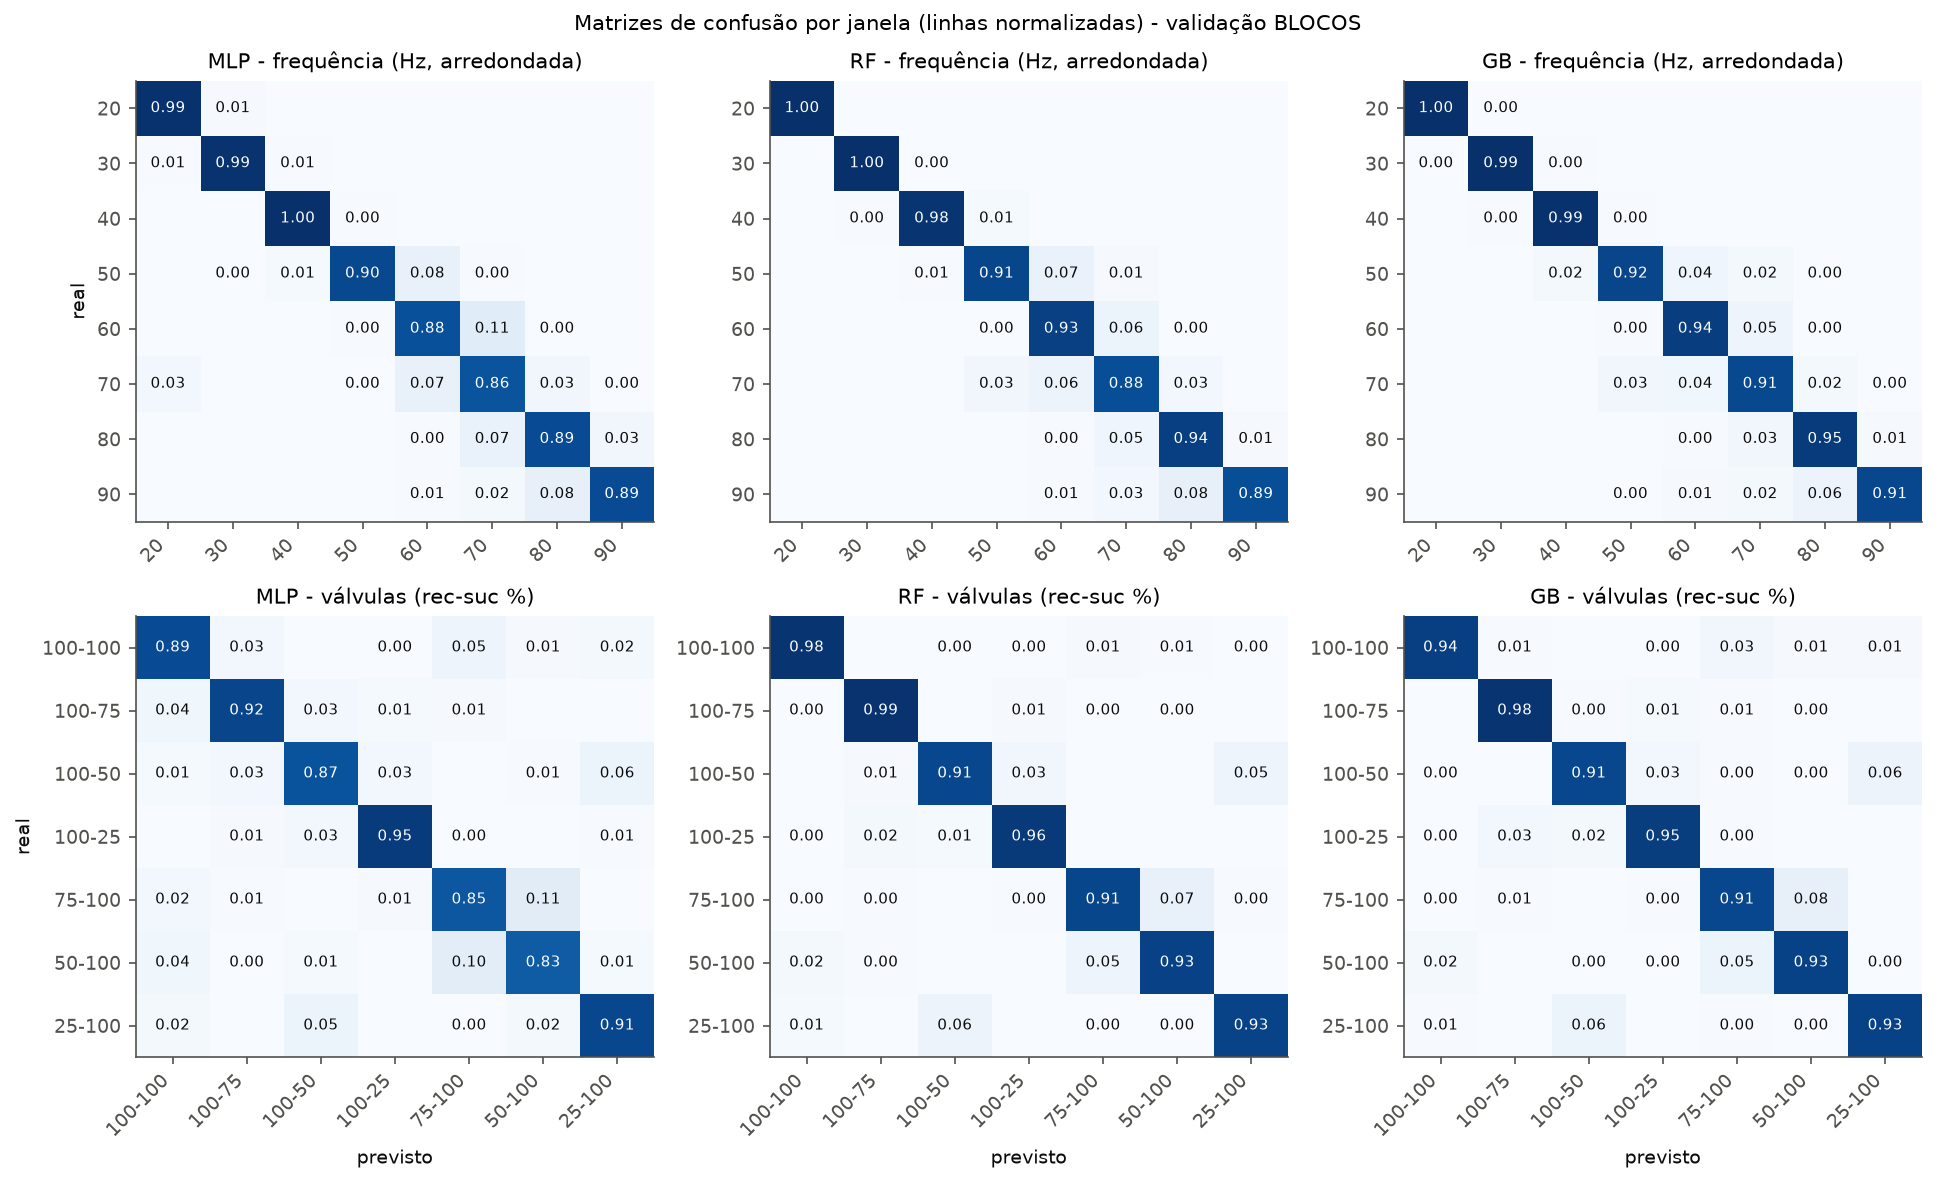
\includegraphics[width=\textwidth]{fig_confusao_BLOCOS.png}
	\caption{Matrizes de confusão em BLOCOS (linhas normalizadas): frequência arredondada (acima) e válvulas (abaixo).}
	\label{fig:conf_blocos}
\end{figure}

\begin{figure}[htbp]
	\centering
	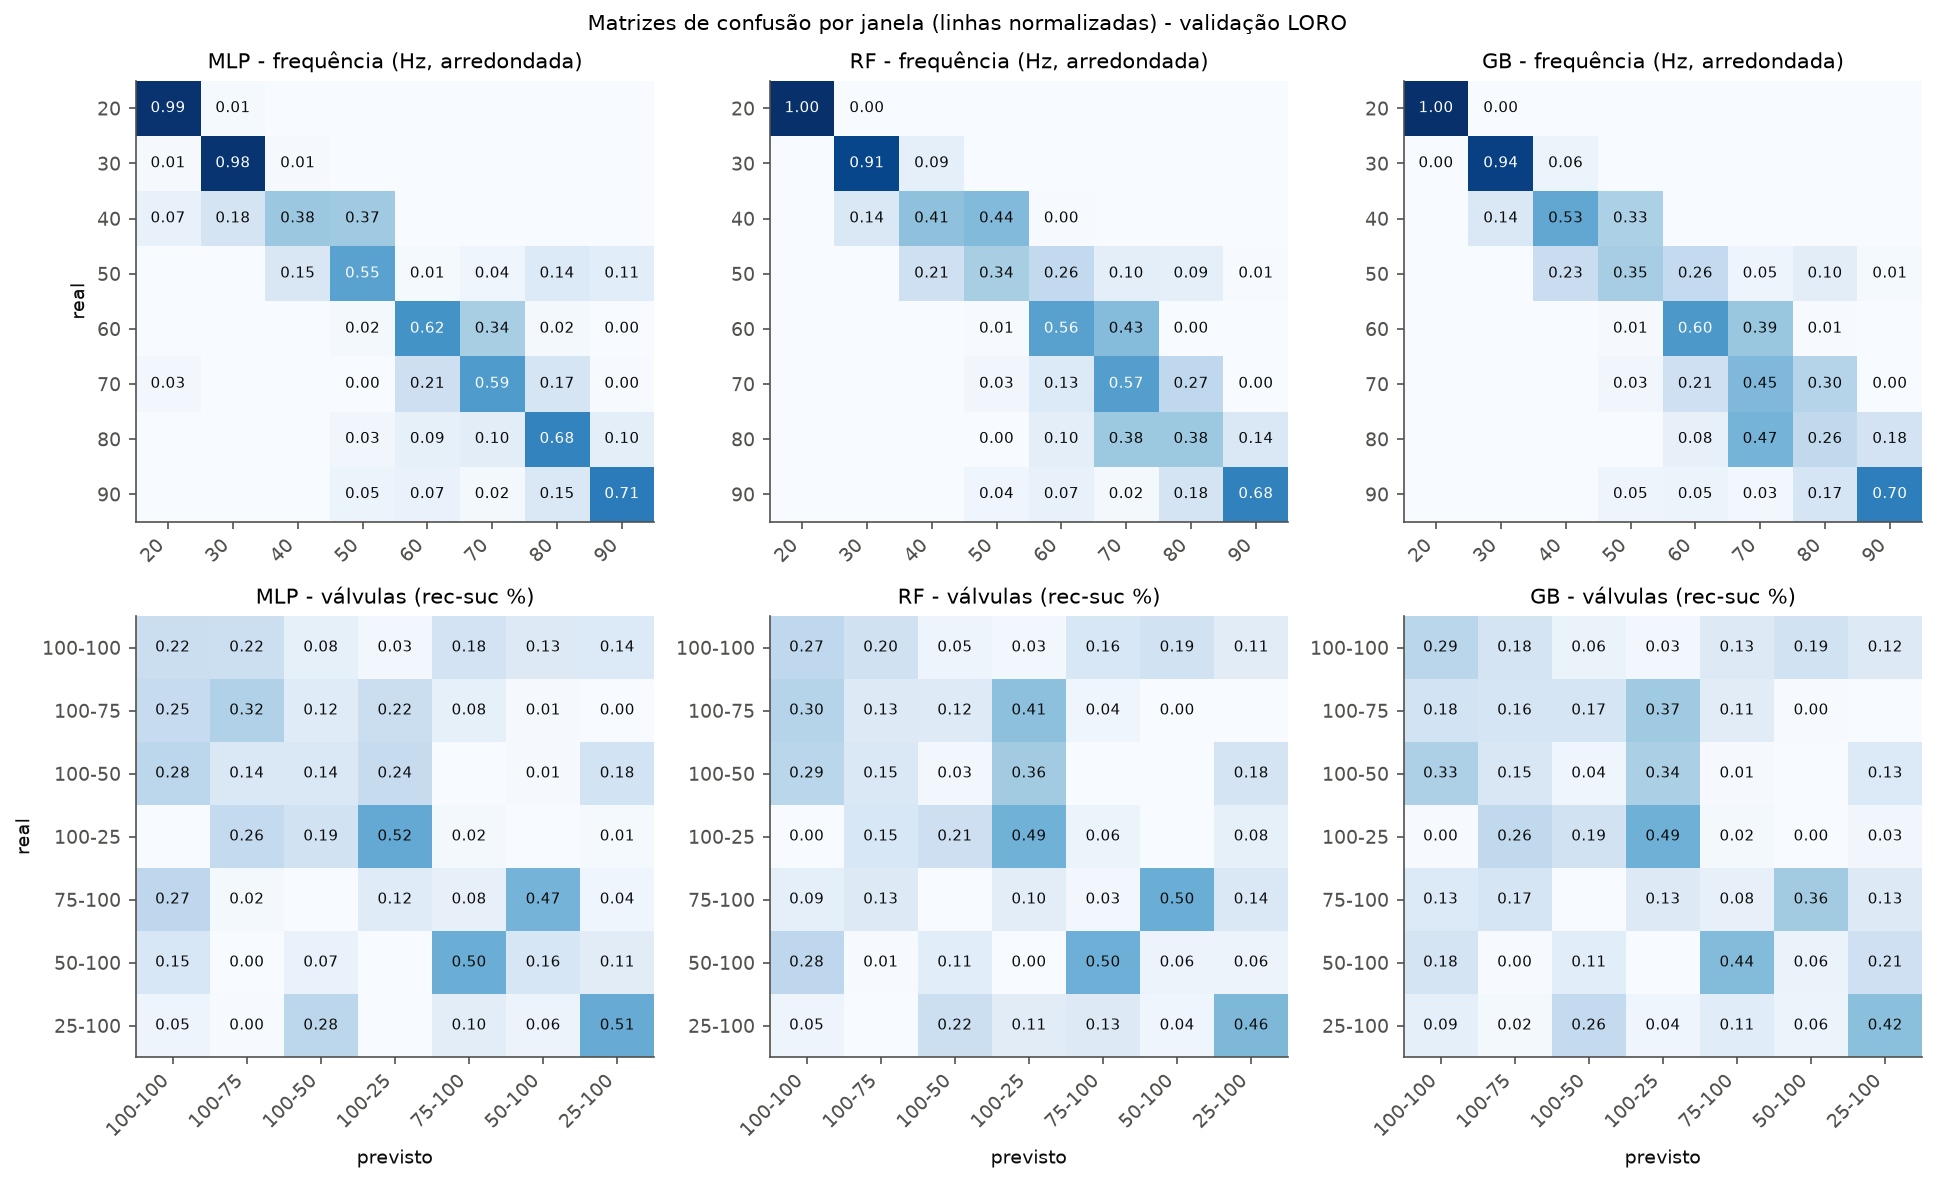
\includegraphics[width=\textwidth]{fig_confusao_LORO.png}
	\caption{Matrizes de confusão em LORO. A diagonal das válvulas praticamente desaparece.}
	\label{fig:conf_loro}
\end{figure}

\begin{figure}[htbp]
	\centering
	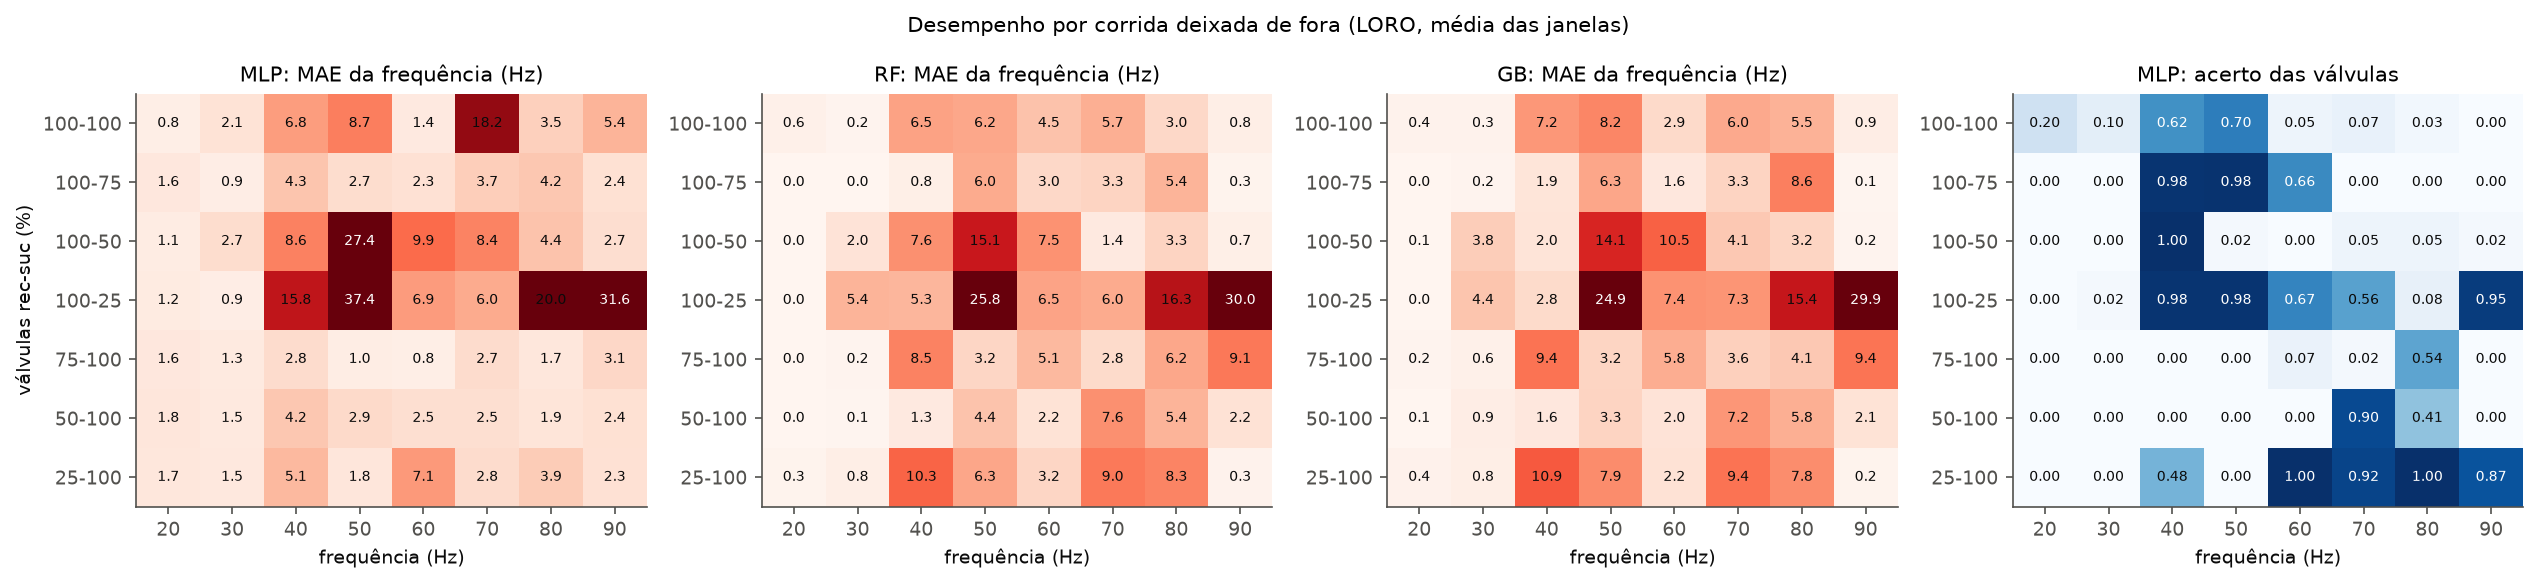
\includegraphics[width=\textwidth]{fig_mapa_LORO.png}
	\caption{Desempenho por corrida deixada de fora: MAE da frequência nos três modelos e acerto das válvulas na MLP.}
	\label{fig:mapa_loro}
\end{figure}

\subsection{Importância dos descritores}

A importância foi medida pela queda de desempenho ao permutar cada descritor nos blocos de teste (Figura~\ref{fig:imp}). Para a frequência, dominam a energia por segundo do canal A, o RA e a amplitude baixa (p10) do canal B e os percentis de energia dos dois canais. Ou seja, o modelo lê o nível de energia contínua, que cresce com a rotação. Para as válvulas, dominam a frequência média e a fração MAXDUR do canal A, além da duração e das contagens dos dois canais, que são descritores de forma e de continuidade do sinal. Pelo resultado em LORO, porém, esses descritores identificam a corrida, e não a válvula. Como os descritores são correlacionados, a permutação individual subestima grupos redundantes, como energia, contagens e duração. A ordem relativa é mais confiável que os valores absolutos.

\begin{figure}[htbp]
	\centering
	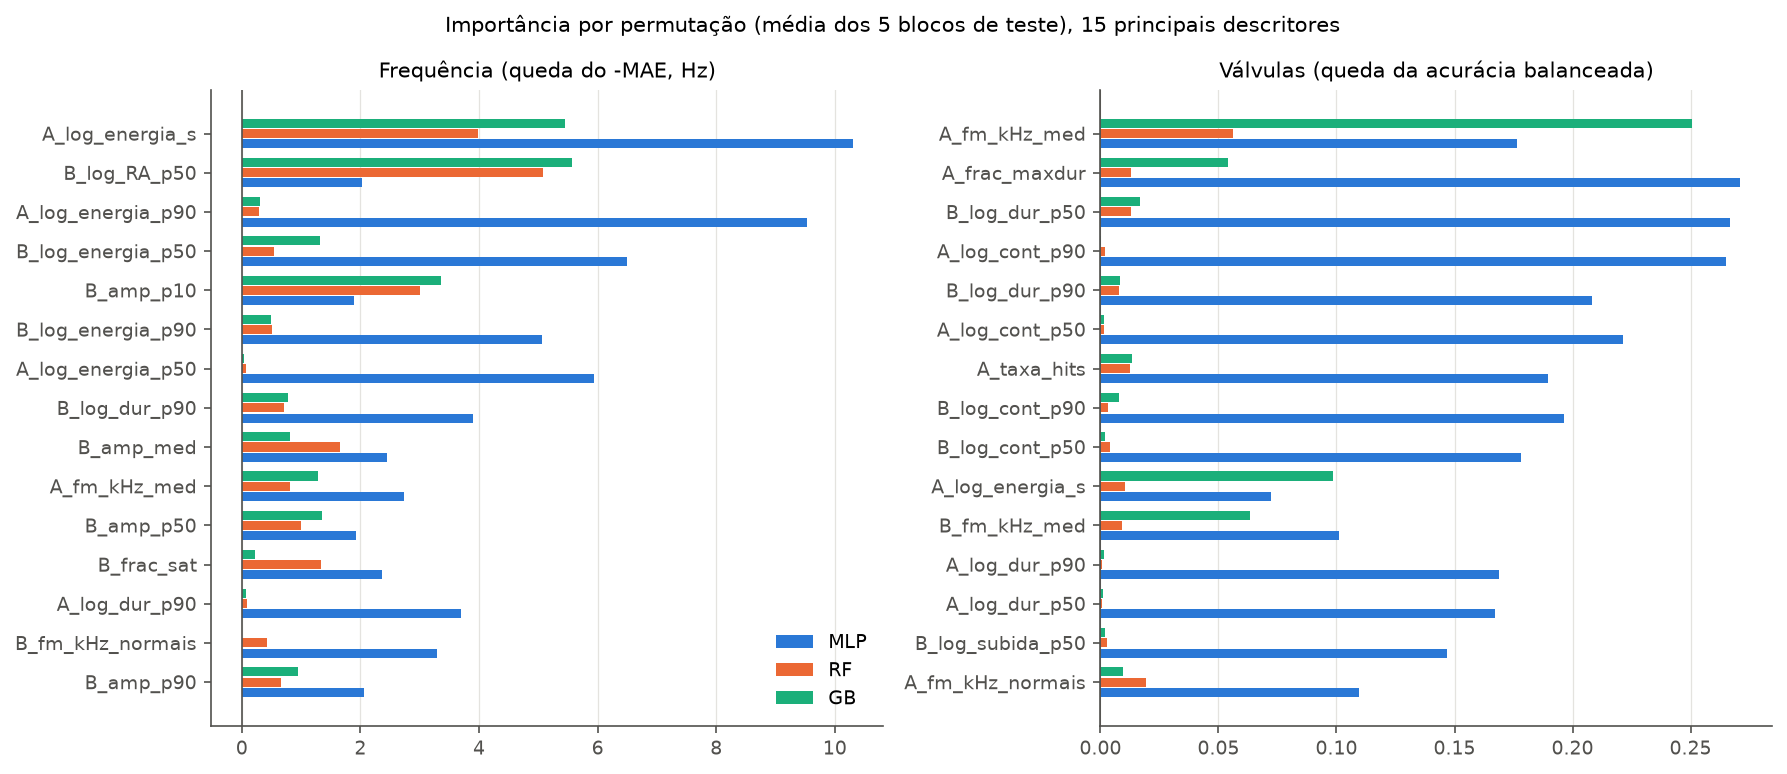
\includegraphics[width=\textwidth]{fig_importancia_descritores.png}
	\caption{Importância por permutação (média dos 5 blocos de teste) dos 15 principais descritores para a frequência e para as válvulas.}
	\label{fig:imp}
\end{figure}

\subsection{Sensibilidade}

Sem o corte comum de limiar, o MAE da frequência mudou menos de 0,2\,Hz e a acurácia das válvulas menos de 1 ponto percentual, como esperado de um corte que remove 0,001\,\% dos \textit{hits}. Com janelas de 2\,s, a MLP melhorou um pouco: acerto do nível em LORO de 72\,\%, ou 79\,\% por corrida. RF e GB pioraram (MAE de 5,6 a 5,7\,Hz), porque cada janela passa a ter cerca de 20 \textit{hits} por canal e os percentis ficam mais ruidosos (Figura~\ref{fig:sens}). Nenhuma variante altera as conclusões.

\begin{figure}[htbp]
	\centering
	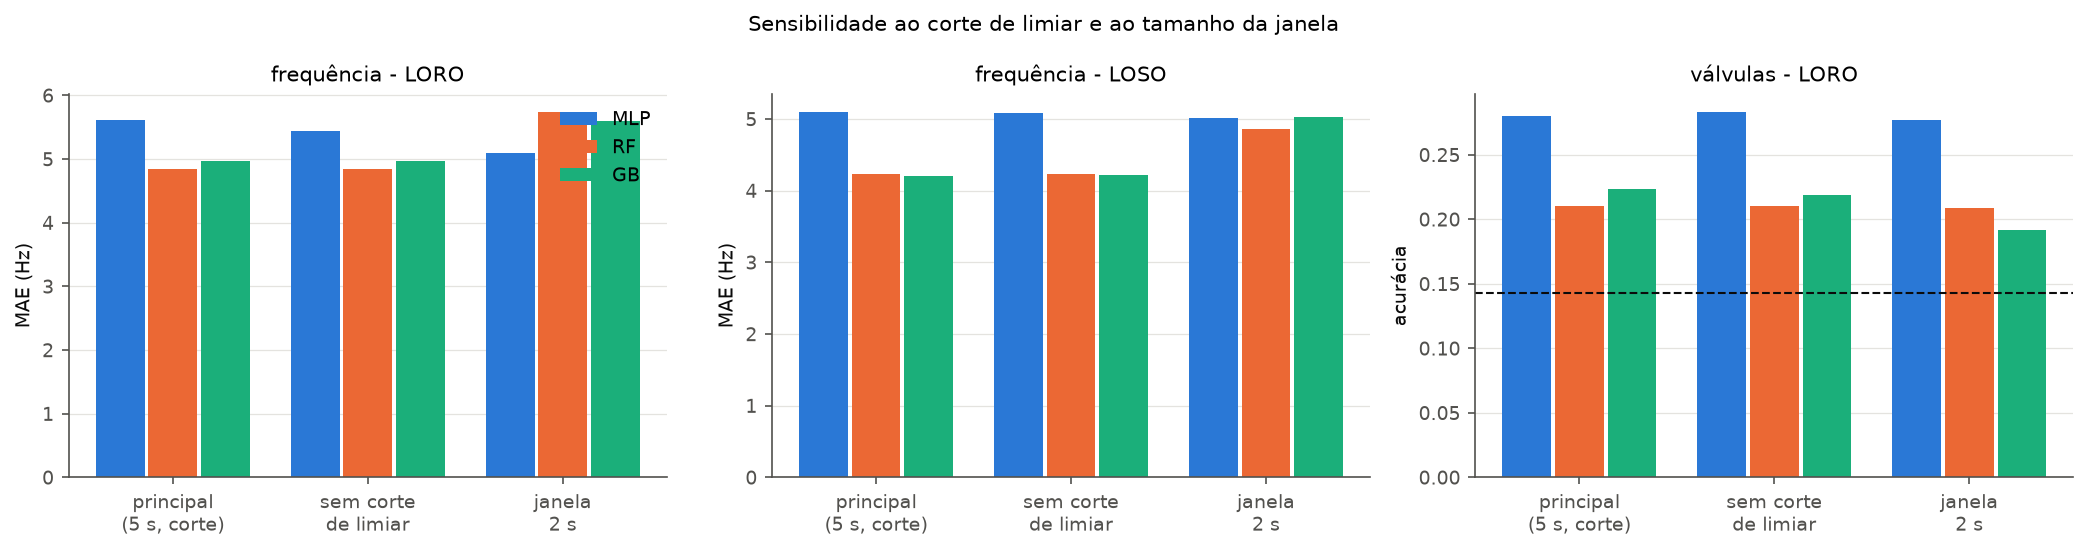
\includegraphics[width=\textwidth]{fig_sensibilidade.png}
	\caption{Sensibilidade ao corte de limiar e ao tamanho da janela, em LORO e LOSO.}
	\label{fig:sens}
\end{figure}

% =======================================================================================================
\section{Verificação não supervisionada}
\label{sec:naosup}

Para checar se a estrutura dos dados acompanha os fatores sem usar rótulos, aplicou-se o \textit{k}-means aos 36 descritores padronizados, com \(k \in \{2, 3, 7, 8, 14, 56\}\). Os agrupamentos foram comparados aos fatores pelo índice de Rand ajustado (ARI) \cite{hubert1985} e pela informação mútua normalizada (NMI).

\begin{table}[htbp]
	\centering
	\caption{ARI entre os agrupamentos do \textit{k}-means e os fatores (0 = acaso; 1 = partição idêntica).}
	\label{tab:ari}
	\small
	\begin{tabular}{rrrrrr}
		\toprule
		\(\boldsymbol{k}\) & \textbf{Frequência} & \textbf{Válvulas} & \textbf{Corrida} & \textbf{Dia} & \textbf{Limiar} \\
		\midrule
		2 & 0,163 & 0,002 & 0,024 & 0,007 & 0,010 \\
		3 & 0,202 & 0,094 & 0,055 & 0,012 & \(-\)0,007 \\
		7 & 0,309 & 0,095 & 0,110 & 0,035 & 0,011 \\
		8 & 0,310 & 0,096 & 0,110 & 0,035 & 0,011 \\
		14 & 0,309 & 0,145 & 0,205 & 0,038 & 0,063 \\
		56 & 0,200 & 0,124 & 0,465 & 0,023 & 0,034 \\
		\bottomrule
	\end{tabular}
\end{table}

A estrutura dominante é a frequência, com ARI de 0,31 para \(k = 8\) (Tabela~\ref{tab:ari}, Figuras~\ref{fig:pca} a~\ref{fig:naosup}). A primeira componente principal explica 56\,\% da variância e separa as janelas de 20 e 30\,Hz, sem saturação, das de 40\,Hz ou mais, saturadas. As válvulas quase não aparecem (ARI \(\approx 0{,}1\)). Com \(k = 56\), os grupos coincidem bastante com as corridas (ARI = 0,47), o que confirma, sem rótulos, a assinatura de corrida vista nos modelos supervisionados. O ARI contra o dia e contra o limiar é próximo de zero: a sessão não domina a estrutura global, embora possa pesar na separação fina entre corridas.

\begin{figure}[htbp]
	\centering
	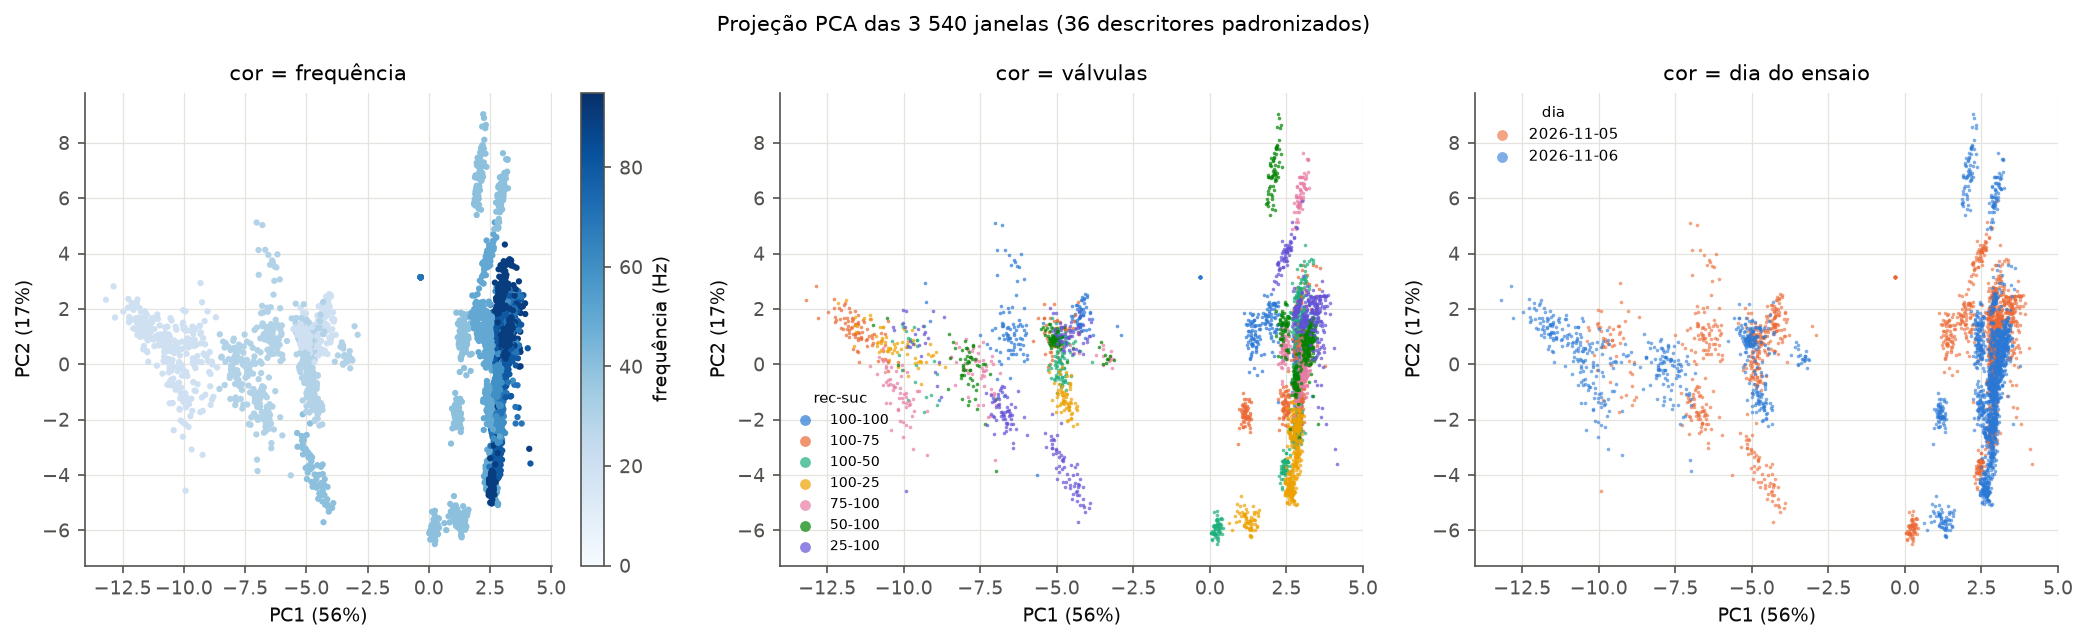
\includegraphics[width=\textwidth]{fig_pca.png}
	\caption{Projeção PCA das 3\,540 janelas, colorida por frequência, por válvula e por dia do ensaio.}
	\label{fig:pca}
\end{figure}

\begin{figure}[htbp]
	\centering
	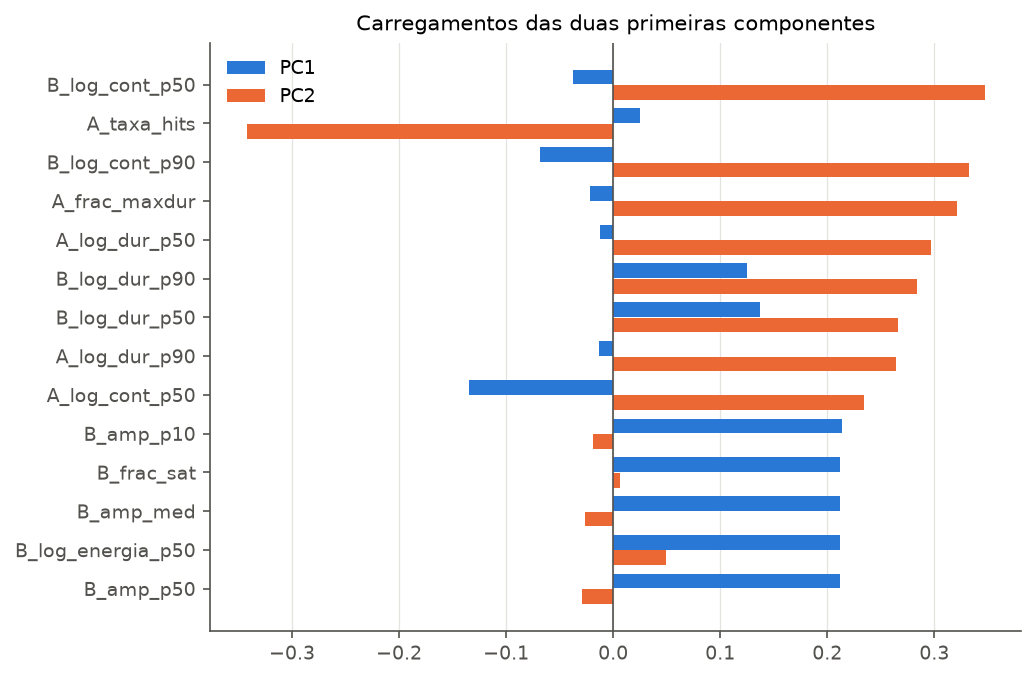
\includegraphics[width=0.7\textwidth]{fig_pca_carregamentos.png}
	\caption{Carregamentos dos descritores nas duas primeiras componentes principais.}
	\label{fig:pca_load}
\end{figure}

\begin{figure}[htbp]
	\centering
	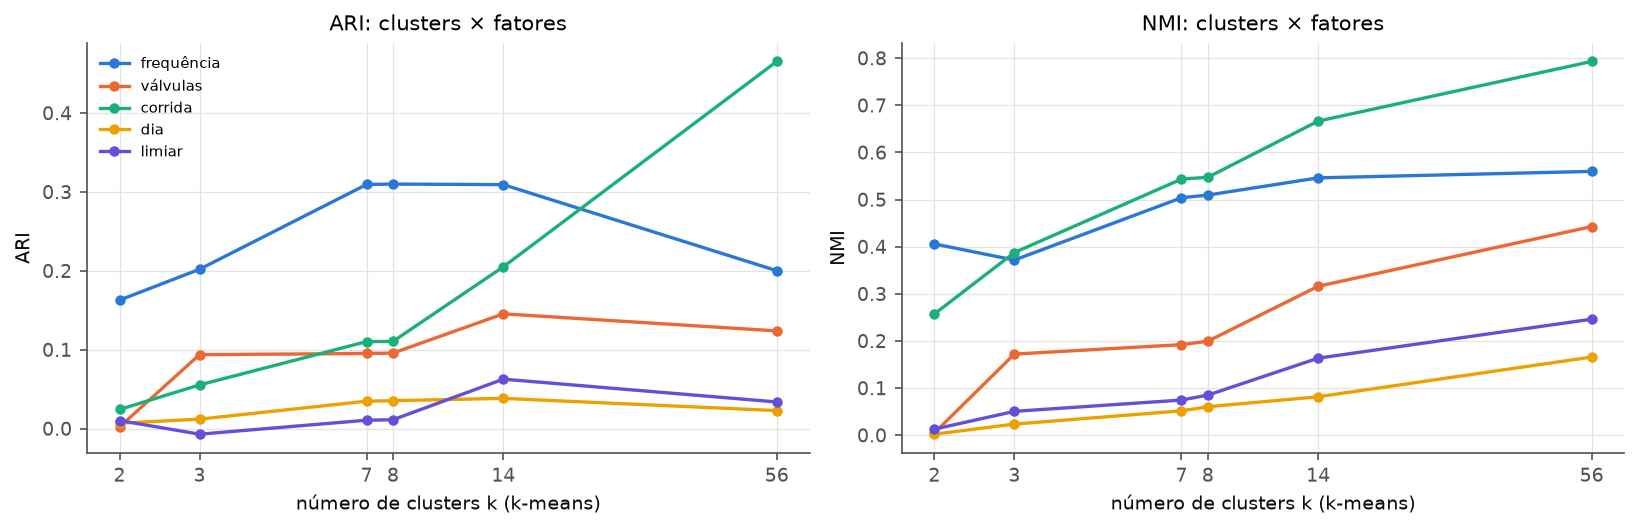
\includegraphics[width=\textwidth]{fig_kmeans_ari.png}
	\caption{ARI e NMI entre os agrupamentos do \textit{k}-means e cada fator, em função de \(k\).}
	\label{fig:ari}
\end{figure}

\begin{figure}[htbp]
	\centering
	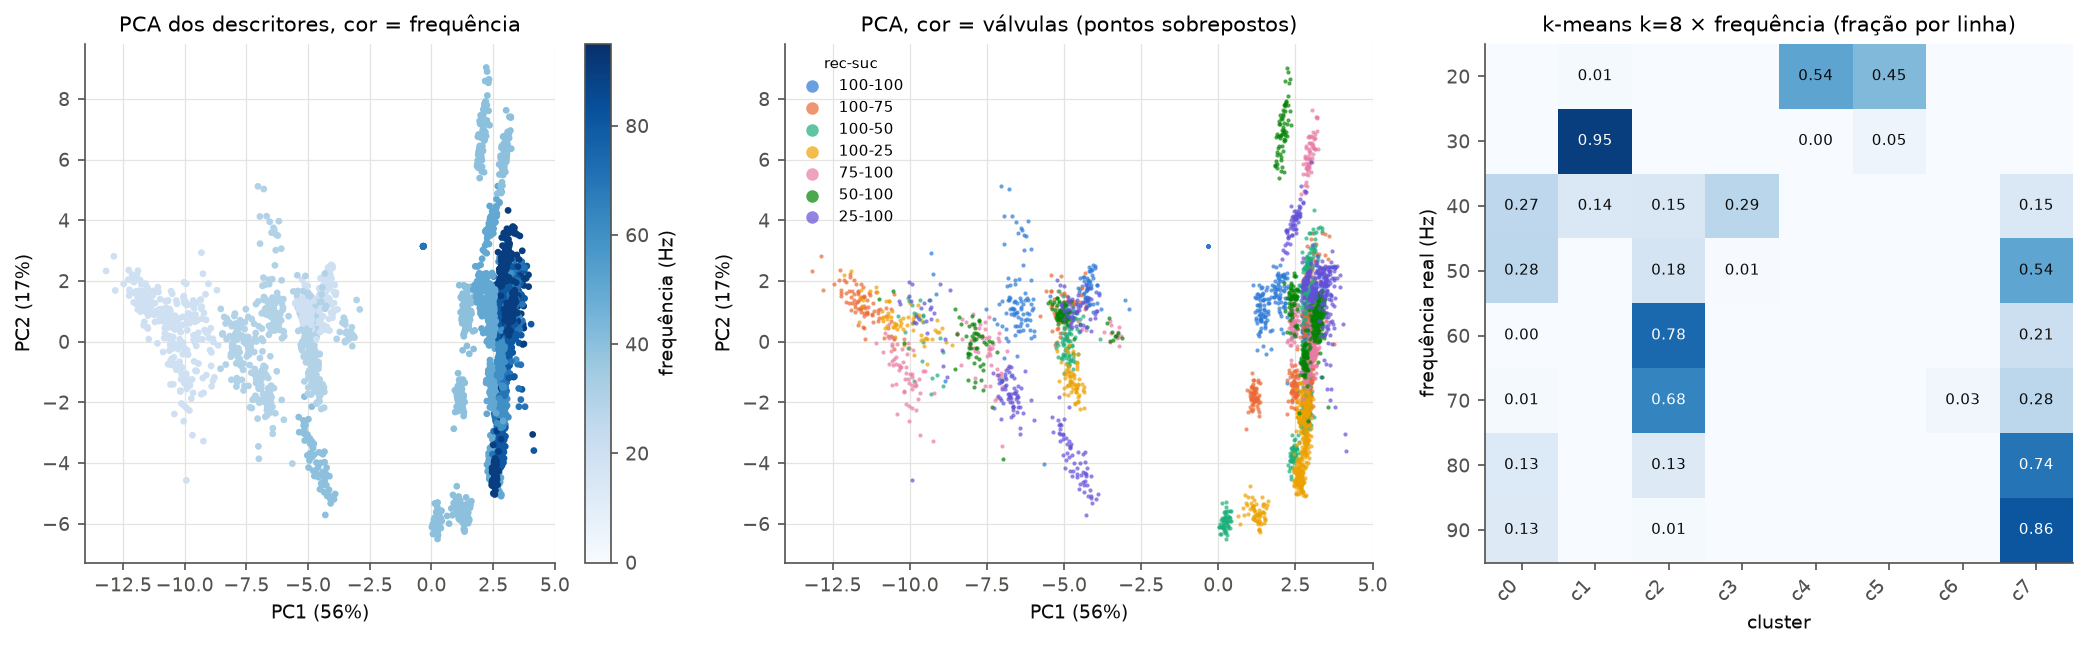
\includegraphics[width=\textwidth]{fig_nao_supervisionado.png}
	\caption{PCA e tabela de contingência entre os grupos do \textit{k}-means (\(k = 8\)) e a frequência.}
	\label{fig:naosup}
\end{figure}

% =======================================================================================================
\section{Discussão e limitações}
\label{sec:discussao}

\paragraph{O que os dados sustentam.} Os descritores de \textit{hits} do MOMEA, agregados em janelas, permitem estimar a frequência do motor com erro de cerca de 5\,Hz em condições e sessões não vistas, e com acerto de \(\pm 10\)\,Hz em mais de 92\,\% das janelas. O sinal útil é essencialmente o nível de energia contínua e a forma dos \textit{hits}. A estimativa é mais precisa abaixo de 40\,Hz, onde não há saturação.

\paragraph{O que os dados não sustentam.} Não é possível afirmar que a configuração das válvulas seja reconhecível a partir destes dados. O desempenho alto em BLOCOS é um artefato da presença da corrida no treino, e o LORO derruba a acurácia para perto do acaso. O resultado também não prova que as válvulas não tenham assinatura de EA. Com uma corrida por condição e as séries ensaiadas em blocos contínuos, o efeito da válvula está confundido com o dia, o horário, a temperatura e o limiar.

\paragraph{Validação interna da MLP.} A parada antecipada da MLP usa 15\,\% das janelas do treino, sorteadas. Essas janelas têm vizinhas da mesma corrida no treino efetivo. Na classificação das válvulas, a validação interna indicou cerca de 90\,\% de acurácia nos folds LORO, enquanto o teste deu 18\,\% (Figura~\ref{fig:val_int}). Isso não contamina o teste, que é sempre externo ao fold. Mas significa que a parada antecipada escolhe a época que melhor reconhece corridas já vistas. Uma validação interna por corrida inteira seria mais coerente com a pergunta.

\begin{figure}[htbp]
	\centering
	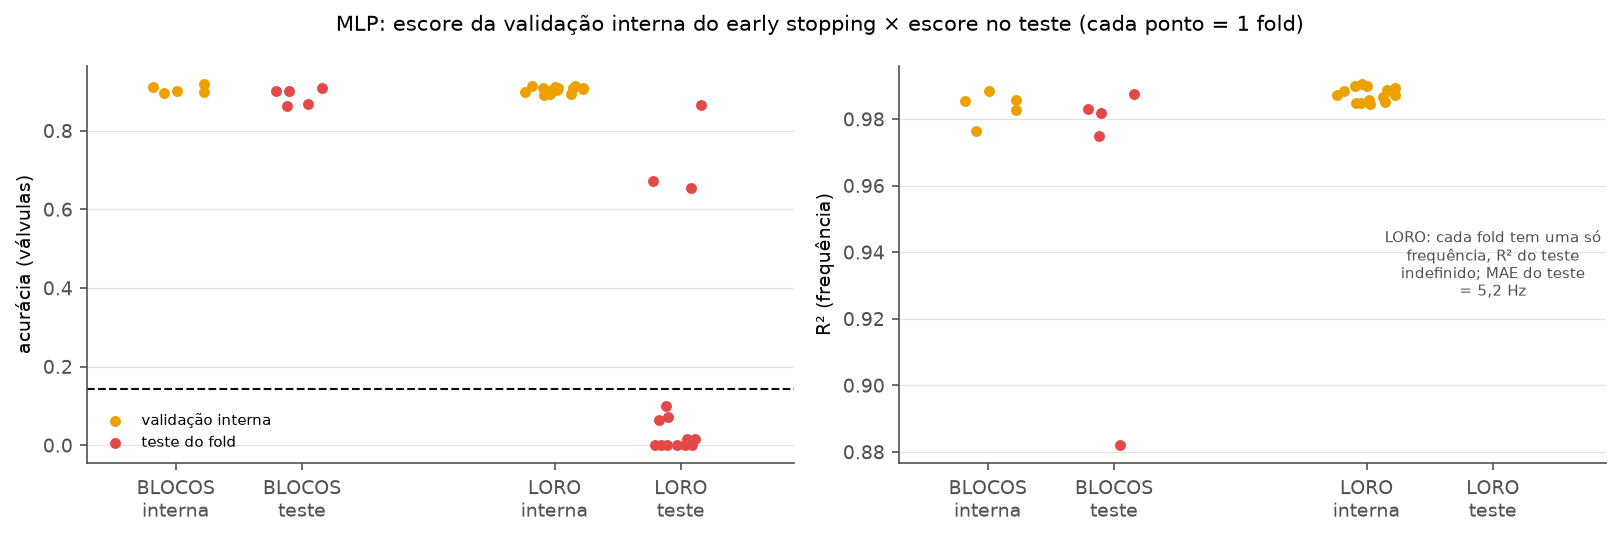
\includegraphics[width=\textwidth]{fig_validacao_interna_vs_teste.png}
	\caption{MLP: escore da validação interna da parada antecipada (janelas sorteadas dentro do treino) \(\times\) escore no teste do fold. Em LORO, foram usados 14 dos 56 folds.}
	\label{fig:val_int}
\end{figure}

\paragraph{Saturação do conversor e filtragem.} Com o ganho de 34\,dB do pré-amplificador (fator 50), a faixa calibrada do conversor A/D, de \(\pm 6{,}3\) a \(\pm 6{,}9\)\,V na entrada da placa, corresponde a 126 a 138\,mV no sensor, ou seja, 102,0 a 102,8\,dB\(_{\mathrm{AE}}\) referidos à entrada. Nos ensaios na bomba, 69,8\,\% dos \textit{hits} atingiram esse limite. A partir de 40 a 50\,Hz de rotação, praticamente todos saturaram (Figuras~\ref{fig:exemplo}, \ref{fig:amplitude} e~\ref{fig:mapas}). Nessa faixa, a amplitude de pico deixou de distinguir as condições de operação. A energia, calculada sobre o sinal recortado, também ficou truncada: a energia por segundo do canal A praticamente estabiliza acima de 60\,Hz (Figura~\ref{fig:mapas}). Isso explica parte da confusão entre níveis vizinhos de 40 a 90\,Hz (Figuras~\ref{fig:conf_loro} e~\ref{fig:conf_loso}) e o melhor desempenho em 20 e 30\,Hz, sem saturação. Recomenda-se reduzir o ganho ou adotar o estágio de ganho ajustável previsto. Recomenda-se também estudar filtros passa-banda que separem o ruído hidráulico e mecânico da bomba, concentrado em frequências mais baixas, das componentes de alta frequência associadas a vórtices e à cavitação incipiente \cite{neill1997,alfayez2005}. Como os ensaios atuais não dispõem de referência independente do estado de cavitação, essa separação permanece uma hipótese a ser verificada.

\paragraph{Limitações.}
\begin{enumerate}
	\item \textbf{Sem repetições.} Não há como estimar a variabilidade entre repetições nem validar deixando uma repetição de fora. O BLOCOS é otimista por construção. O LORO é a estimativa honesta, mas cada fold testa uma única corrida.
	\item \textbf{Ordem fixa e deriva.} Válvulas, dia, horário e limiar estão confundidos. Para a frequência, o LOSO e o teste entre dias mostram robustez à troca de sessão. Para as válvulas, isso não pode ser testado.
	\item \textbf{Limiar variável} (50 a 65\,dB\(_{\mathrm{AE}}\)). Duração, contagens e energia foram medidas acima de limiares diferentes, sem correção possível.
	\item \textbf{Cadência imposta pelo rearme} (cerca de 10 \textit{hits}/s por canal) e ROVL sempre ativo. Os \textit{hits} são uma amostragem de um sinal contínuo, e a taxa de \textit{hits} não é um descritor físico.
	\item \textbf{Saturação a partir de 40\,Hz} (limite de 102,0 a 102,8\,dB\(_{\mathrm{AE}}\) com 34\,dB de ganho). A amplitude e a energia perdem informação justamente na faixa em que as condições mais se confundem; ver o parágrafo sobre saturação e filtragem.
	\item \textbf{Dependência entre janelas.} As métricas por janela inflam o número efetivo de amostras. A unidade independente é a corrida (56).
	\item \textbf{Hiperparâmetros fixos.} Os resultados são linhas de base, e não desempenho otimizado.
\end{enumerate}

\paragraph{Recomendações para o próximo ensaio.}
\begin{itemize}
	\item Repetir cada condição pelo menos 2 ou 3 vezes, em ordem aleatorizada ou em blocos aleatorizados por dia, voltando a condições já ensaiadas. Só assim é possível validar com uma repetição deixada de fora e separar o efeito da válvula da deriva.
	\item Manter ganho e limiar fixos em todas as sessões, reduzir o ganho (ou usar o estágio de ganho ajustável) para evitar a saturação acima de 40\,Hz e avaliar filtros passa-banda, como discutido acima.
	\item Confirmar no HDL o limite do bloqueio re-armável e, para sinal contínuo, complementar os \textit{hits} com descritores de nível, como RMS e energia por intervalo fixo, ou com bandas espectrais \cite{derakhshan1991}.
	\item Reservar uma campanha futura inteira como teste final bloqueado, fora do tempo, avaliado uma única vez.
\end{itemize}

% =======================================================================================================
\section{Conclusões}
\label{sec:conclusoes}

Com 56 corridas de um delineamento cruzado de frequência e válvulas, os descritores de \textit{hits} do MOMEA agregados em janelas de 5\,s estimaram a frequência do motor com MAE de 4,2 a 5,6\,Hz para condições e sessões não vistas. MLP, RF e GB tiveram desempenho semelhante. A configuração das válvulas só foi reconhecida quando a própria corrida estava no treino. Com a corrida deixada de fora, a acurácia ficou em 21 a 28\,\% (acaso: 14\,\%). A diferença entre as validações é o principal resultado metodológico: em dados de EA com uma corrida por condição e ordem fixa de ensaio, dividir \textit{hits} ou janelas ao acaso, ou mesmo em blocos dentro da corrida, superestima a capacidade de classificação. Ensaios com repetições aleatorizadas, ganho e limiar fixos e descritores contínuos são necessários para avaliar a detecção de condições ligadas às válvulas e à cavitação.

% =======================================================================================================
\begin{thebibliography}{99}

	\bibitem[Alfayez et al.(2005)]{alfayez2005}
	ALFAYEZ, L.; MBA, D.; DYSON, G.
	\newblock The application of acoustic emission for detecting incipient cavitation and the best efficiency point of a 60 kW centrifugal pump: case study.
	\newblock \emph{NDT \& E International}, v. 38, n. 5, p. 354--358, 2005.
	\newblock DOI: \href{https://doi.org/10.1016/j.ndteint.2004.10.002}{10.1016/j.ndteint.2004.10.002}.

	\bibitem[Breiman(2001)]{breiman2001}
	BREIMAN, L.
	\newblock Random forests.
	\newblock \emph{Machine Learning}, v. 45, n. 1, p. 5--32, 2001.
	\newblock DOI: \href{https://doi.org/10.1023/A:1010933404324}{10.1023/A:1010933404324}.

	\bibitem[Brennen(1995)]{brennen1995}
	BRENNEN, C. E.
	\newblock \emph{Cavitation and Bubble Dynamics}.
	\newblock New York: Oxford University Press, 1995.

	\bibitem[Derakhshan et al.(1991)]{derakhshan1991}
	DERAKHSHAN, O.; HOUGHTON, J. R.; JONES, R. K.; MARCH, P. A.
	\newblock Cavitation monitoring of hydroturbines with RMS acoustic emission measurement.
	\newblock In: \emph{ASTM Special Technical Publication 1077}.
	\newblock Philadelphia: ASTM, 1991. p. 305--315.
	\newblock DOI: \href{https://doi.org/10.1520/STP19102S}{10.1520/STP19102S}.

	\bibitem[Friedman(2001)]{friedman2001}
	FRIEDMAN, J. H.
	\newblock Greedy function approximation: a gradient boosting machine.
	\newblock \emph{The Annals of Statistics}, v. 29, n. 5, p. 1189--1232, 2001.
	\newblock DOI: \href{https://doi.org/10.1214/aos/1013203451}{10.1214/aos/1013203451}.

	\bibitem[Hubert e Arabie(1985)]{hubert1985}
	HUBERT, L.; ARABIE, P.
	\newblock Comparing partitions.
	\newblock \emph{Journal of Classification}, v. 2, n. 1, p. 193--218, 1985.
	\newblock DOI: \href{https://doi.org/10.1007/BF01908075}{10.1007/BF01908075}.

	\bibitem[Kaufman et al.(2012)]{kaufman2012}
	KAUFMAN, S.; ROSSET, S.; PERLICH, C.; STITELMAN, O.
	\newblock Leakage in data mining: formulation, detection, and avoidance.
	\newblock \emph{ACM Transactions on Knowledge Discovery from Data}, v. 6, n. 4, art. 15, 2012.
	\newblock DOI: \href{https://doi.org/10.1145/2382577.2382579}{10.1145/2382577.2382579}.

	\bibitem[Neill et al.(1997)]{neill1997}
	NEILL, G. D.; REUBEN, R. L.; SANDFORD, P. M.; BROWN, E. R.; STEEL, J. A.
	\newblock Detection of incipient cavitation in pumps using acoustic emission.
	\newblock \emph{Proceedings of the Institution of Mechanical Engineers, Part E: Journal of Process Mechanical Engineering}, v. 211, n. 4, p. 267--277, 1997.
	\newblock DOI: \href{https://doi.org/10.1243/0954408971529737}{10.1243/0954408971529737}.

	\bibitem[Ohno e Ohtsu(2010)]{ohno2010}
	OHNO, K.; OHTSU, M.
	\newblock Crack classification in concrete based on acoustic emission.
	\newblock \emph{Construction and Building Materials}, v. 24, n. 12, p. 2339--2346, 2010.
	\newblock DOI: \href{https://doi.org/10.1016/j.conbuildmat.2010.05.004}{10.1016/j.conbuildmat.2010.05.004}.

	\bibitem[Pedregosa et al.(2011)]{pedregosa2011}
	PEDREGOSA, F. et al.
	\newblock Scikit-learn: machine learning in Python.
	\newblock \emph{Journal of Machine Learning Research}, v. 12, p. 2825--2830, 2011.

	\bibitem[Prechelt(1998)]{prechelt1998}
	PRECHELT, L.
	\newblock Early stopping -- but when?
	\newblock In: ORR, G. B.; MÜLLER, K.-R. (ed.). \emph{Neural Networks: Tricks of the Trade}.
	\newblock Berlin: Springer, 1998. (Lecture Notes in Computer Science, v. 1524). p. 55--69.

	\bibitem[Roberts et al.(2017)]{roberts2017}
	ROBERTS, D. R. et al.
	\newblock Cross-validation strategies for data with temporal, spatial, hierarchical, or phylogenetic structure.
	\newblock \emph{Ecography}, v. 40, n. 8, p. 913--929, 2017.
	\newblock DOI: \href{https://doi.org/10.1111/ecog.02881}{10.1111/ecog.02881}.

	\bibitem[Unn{\th}{\'o}rsson(2013)]{unnthorsson2013}
	UNN{\TH}{\'O}RSSON, R.
	\newblock Hit detection and determination in AE bursts.
	\newblock In: SIKORSKI, W. (ed.). \emph{Acoustic Emission---Research and Applications}.
	\newblock Rijeka: IntechOpen, 2013.
	\newblock DOI: \href{https://doi.org/10.5772/54754}{10.5772/54754}.

	\bibitem[Vallen Systeme(2022)]{vallen2022}
	VALLEN SYSTEME GMBH.
	\newblock \emph{AMSY-6: System Specification}.
	\newblock Wolfratshausen: Vallen Systeme GmbH, 2022.

	\bibitem[Varma e Simon(2006)]{varma2006}
	VARMA, S.; SIMON, R.
	\newblock Bias in error estimation when using cross-validation for model selection.
	\newblock \emph{BMC Bioinformatics}, v. 7, art. 91, 2006.
	\newblock DOI: \href{https://doi.org/10.1186/1471-2105-7-91}{10.1186/1471-2105-7-91}.

\end{thebibliography}

\end{document}
